\documentclass[10pt,twocolumn,letterpaper]{article}

\usepackage{cvpr}
\usepackage{times}
\usepackage{epsfig}
\usepackage{graphicx}
\usepackage{amsmath}
\usepackage{amssymb}
\usepackage{url}
\usepackage{subcaption}
\usepackage{listings}
\usepackage{float}
\usepackage{multirow}
\usepackage{booktabs}


\lstset{
    basicstyle=\ttfamily\small,
    breaklines=true,         
    frame=single,
    language=C++,
    showstringspaces=false
}

% Include other packages here, before hyperref.

% If you comment hyperref and then uncomment it, you should delete
% egpaper.aux before re-running latex.  (Or just hit 'q' on the first latex
% run, let it finish, and you should be clear).
%\usepackage[pagebackref=true,breaklinks=true,letterpaper=true,colorlinks,bookmarks=false]{hyperref}

\cvprfinalcopy % *** Uncomment this line for the final submission

\def\cvprPaperID{****} % *** Enter the CVPR Paper ID here
\def\httilde{\mbox{\tt\raisebox{-.5ex}{\symbol{126}}}}

% Pages are numbered in submission mode, and unnumbered in camera-ready
\ifcvprfinal\pagestyle{empty}\fi
\begin{document}

%%%%%%%%% TITLE
\title{Parallel Morphological Image Processing}

\author{Davide Lombardi\\
E-mail address\\
{\tt\small davide.lombardi2@edu.unifi.it}
% For a paper whose authors are all at the same institution,
% omit the following lines up until the closing ``}''.
% Additional authors and addresses can be added with ``\and'',
% just like the second author.
% To save space, use either the email address or home page, not both
}
\maketitle
\thispagestyle{empty}

%%%%%%%%% ABSTRACT
\begin{abstract}
Morphological Image Processing is a tool for feature extraction and image restoration. However, processing high-resolution imagery with standard 2D stencils introduces severe computational bottlenecks. This project presents an optimized, parallelized framework using C++17 and OpenMP to accelerate morphological operations. By transitioning from quadratic $O(K^2)$ 2D stencils to linear $O(2K)$ 1D separable kernels, and leveraging a producer-consumer pipeline architecture for compound operations, I achieve significant performance gains. Benchmarked on the BSDS500 dataset, the optimal parallel implementation achieves a peak speedup of approximately 22x for $15 \times 15$ kernels compared to a standard sequential baseline.
\end{abstract}

%%%%%%%%% BODY TEXT
\noindent\large\textbf{Future Distribution Permission}

The author(s) of this report give permission for this document to be distributed to Unifi-affiliated students taking future courses.

\section{Introduction}
Mathematical Morphology (MM) provides a robust mathematical framework for analyzing geometric structures within images \cite{wikipedia_mm, opencv_morph}. Fundamental operations rely on probing an input image with a Structuring Element (SE) to extract critical region descriptors such as boundaries, skeletons, and convex hulls \cite{opencv_morph, ismail_paper}. While highly effective for tasks like noise reduction and edge detection, the standard implementation of these transformations scales quadratically with the kernel size $K$, resulting in an $O(K^2)$ time complexity. As modern computer vision applications increasingly demand real-time processing of high-resolution datasets like the \textbf{BSDS500}, sequential execution becomes prohibitively slow.

To address this limitation, this study investigates advanced algorithmic and hardware-level optimizations. Rather than relying solely on standard multi-threading, I explored a multi-tiered approach. First, I reduced the theoretical algorithmic complexity by utilizing \textbf{1D separable kernels}. Second, I managed the strict sequential dependencies inherent in compound operations (e.g., Opening and Closing) by implementing a \textbf{Producer-Consumer pipeline} architecture. Through these combined strategies, this paper provides a rigorous evaluation of speedup and efficiency across modern multi-core CPU architectures.

\section{Mathematical Formulation}
This project focuses on grayscale morphology utilizing flat structuring elements. In this context, morphological operators function as order statistics filters \cite{wikipedia_mm, ismail_paper}. Let $f(x)$ represent the input image and $B$ denote the support of the structuring element.

\subsection{Fundamental Operators}
The two primary non-linear operators are \textbf{Erosion} and \textbf{Dilation}:

\begin{itemize}
    \item \textbf{Erosion ($\ominus$)}: effectively "erodes" the boundaries of foreground objects, reducing their size. It is instrumental in discarding small-scale noise and detaching overlapping structures \cite{opencv_morph, ismail_paper}. Mathematically, it returns the minimum value in the neighborhood defined by $B$:
    \begin{equation}
    (f \ominus b)(x) = \inf_{z \in B} f(x+z)
    \end{equation}
    
    \item \textbf{Dilation ($\oplus$)}: acts as the dual of erosion, expanding foreground regions. It is widely used to fill gaps and join broken segments of a digital object \cite{opencv_morph, ismail_paper}. It returns the maximum value in the neighborhood:
    \begin{equation}
    (f \oplus b)(x) = \sup_{z \in B} f(x+z)
    \end{equation}
\end{itemize}

\begin{figure}[htpb]
    \centering
    \begin{subfigure}[b]{0.32\linewidth}
        \centering
        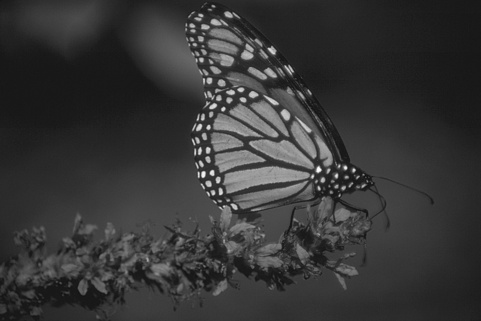
\includegraphics[width=\textwidth]{img/original.png}
        \caption{Original}
        \label{fig:orig}
    \end{subfigure}
    \hfill
    \begin{subfigure}[b]{0.32\linewidth}
        \centering
        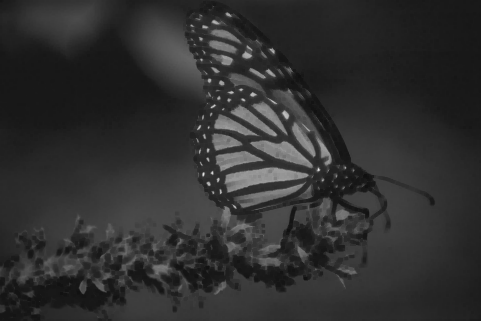
\includegraphics[width=\textwidth]{img/eroded.png}
        \caption{Eroded}
        \label{fig:erod}
    \end{subfigure}
    \hfill
    \begin{subfigure}[b]{0.32\linewidth}
        \centering
        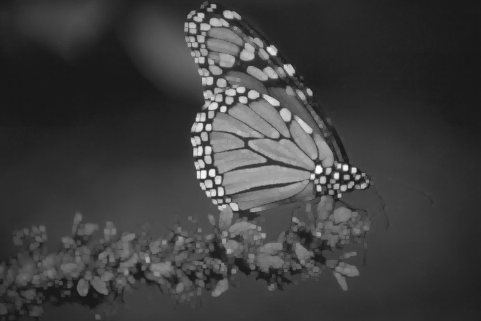
\includegraphics[width=\textwidth]{img/dilated.png}
        \caption{Dilated}
        \label{fig:dilat}
    \end{subfigure}
    
    \caption{Comparison of morphological operations.}
    \label{fig:morph_comparison_base}
\end{figure}

\subsection{Compound Operations}
By combining the fundamental operators, I implemented \textbf{Opening} and \textbf{Closing} for sophisticated image restoration \cite{opencv_morph, wikipedia_mm}:

\begin{itemize}
    \item \textbf{Opening ($\circ$)}: defined as erosion followed by dilation. It is particularly effective for removing small bright noise objects while restoring the original proportions of larger structures \cite{opencv_morph, ismail_paper}:
    \begin{equation}
    f \circ b = (f \ominus b) \oplus b
    \end{equation}
    
    \item \textbf{Closing ($\bullet$)}: defined as dilation followed by erosion. It is essential for filling small dark holes or gaps within bright structures \cite{opencv_morph, ismail_paper}:
    \begin{equation}
    f \bullet b = (f \oplus b) \ominus b
    \end{equation}
\end{itemize}

\begin{figure}[htpb]
    \centering
    \begin{subfigure}[b]{0.32\linewidth}
        \centering
        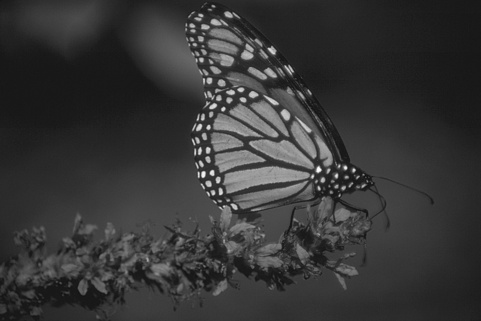
\includegraphics[width=\textwidth]{img/original.png}
        \caption{Original}
        \label{fig:orig2}
    \end{subfigure}
    \hfill
    \begin{subfigure}[b]{0.32\linewidth}
        \centering
        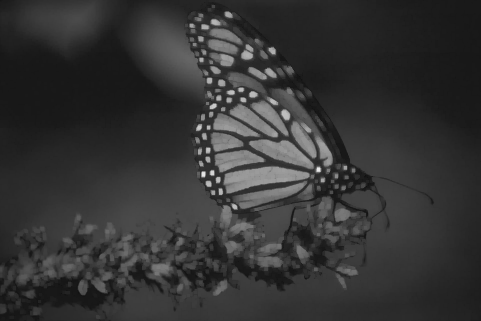
\includegraphics[width=\textwidth]{img/opening.png}
        \caption{Opening}
        \label{fig:open}
    \end{subfigure}
    \hfill
    \begin{subfigure}[b]{0.32\linewidth}
        \centering
        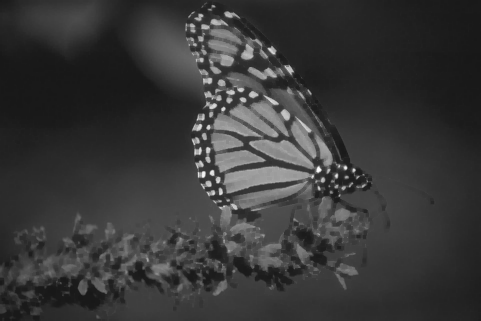
\includegraphics[width=\textwidth]{img/closing.png}
        \caption{Closing}
        \label{fig:close}
    \end{subfigure}
    
   \caption{Application of compound operations.}
   \label{fig:opening_closing}
\end{figure}
\vspace{3cm}

\section{Implementation Details}
In this section, I describe the software implementation of the morphological processing framework. It details the reference dataset and its preprocessing stages, the strategic utilization of OpenMP directives for parallelization and vectorization and the logical architecture of both the sequential baseline and the advanced parallel optimizations.

\subsection{Dataset and Preprocessing}
For all experiments, I utilized the \textbf{BSDS500} (Berkeley Segmentation Dataset), a widely adopted benchmark in image processing research. This dataset provides a heterogeneous benchmark of real-world images, which is ideal for testing the robustness of stencil computing algorithms under realistic application workloads, such as boundary segmentation.
The first 200 images are extracted from the dataset to establish the core evaluation workload. The original images feature base dimensions of either $321 \times 481$ or $481 \times 321$ pixels, depending on whether they are captured in landscape or portrait orientation, providing a uniform baseline before scaling transformations are applied.
The data preparation pipeline is orchestrated via an automated Python script and consists of two main preprocessing phases:
\begin{itemize}
    \item \textbf{Grayscale Conversion}: each image is converted from the RGB color space to grayscale. This conversion simplifies the morphological operations by reducing the data to a single intensity channel, focusing the benchmark on pixel-intensity extrema (min/max) within the structuring element.
    \item \textbf{Rescaling}: to systematically evaluate the framework's scalability, the base images were upscaled by factors of 2x and 4x. This multi-scaling approach enables a rigorous analysis of both \textbf{Strong Scaling} and \textbf{Weak Scaling}. 
\end{itemize}

\subsection{OpenMP Directives}
The parallel implementation leverages the \textbf{OpenMP} API to exploit multi-core architectures. In the project, the following OpenMP directives are applied:

\begin{itemize}
    \item \texttt{\#pragma omp parallel for}: used to parallelize the primary loops by partitioning the iteration space among the thread pool.
    \item \texttt{collapse(2)}: applied to nested loops to merge them into a single, larger iteration space, reducing work granularity and improving parallel scalability on images.
    \item \texttt{schedule(static)}: employed to distribute iterations in fixed-size blocks to minimize runtime scheduling overhead.
    \item \texttt{\#pragma omp simd}: integrated to explicitly trigger hardware-level vectorization, leveraging SIMD registers for simultaneous pixel intensity comparisons (min/max) within the inner loops.
    \item \texttt{\#pragma omp atomic write}: used to ensure thread-safe updates to shared variables (e.g., pipeline status flags).
    \item \texttt{\#pragma omp atomic read}: utilized to perform thread-safe loads of shared variables, preventing partial reads in a multi-threaded environment.
\end{itemize}

\subsection{Sequential Algorithm}
\label{subsec:sequential}

The sequential algorithm establishes the baseline for the entire framework. It implements a naive 2D spatial domain stencil execution path, processing pixels one by one without multi-threading or hardware vector extensions.

\subsubsection{Erosion and Dilation}
Erosion and dilation are implemented using a 4-nested loop structure. The two outer loops iterate over the image coordinates $(x, y)$, while the two inner loops scan the local neighborhood defined by the $K \times K$ structuring element (kernel).

To handle pixels near the image boundaries without allocating extra padding memory, an inline clamping policy is utilized. The coordinates are clipped to the valid image domain using \lstinline|std::min| and \lstinline|std::max|, as illustrated in Listing~\ref{lst:fundamental_seq}.

\begin{lstlisting}[language=C++, caption={Sequential implementation of core Erosion and Dilation operators.}, label={lst:fundamental_seq}, basicstyle=\ttfamily\footnotesize, frame=single, breaklines=true]
for (int y = 0; y < h; ++y) {
    for (int x = 0; x < w; ++x) {
        unsigned char min_val = 255;
        unsigned char max_val = 0;

        for (int ky = -offset; ky <= offset; ++ky) {
            for (int kx = -offset; kx <= offset; ++kx) {
                // boundary clamping (zero-overhead padding)
                int nx = std::max(0, std::min(w - 1, x + kx));
                int ny = std::max(0, std::min(h - 1, y + ky));

                unsigned char pixel = input.getPixel(nx, ny);
                min_val = std::min(min_val, pixel); // for Erosion
                max_val = std::max(max_val, pixel); // for Dilation
            }
        }
        output.setPixel(x, y, min_val); // max_val for Dilation
    }
}
\end{lstlisting}

This approach avoids expensive conditional branching (\lstinline|if-else| blocks) inside the critical innermost loop, allowing the CPU execution pipeline to remain clear of branch mispredictions. However, the theoretical computational complexity remains bound to $\mathcal{O}(M \times N \times K^2)$, where $M \times N$ represents the image dimensions and $K$ is the kernel size. 

Furthermore, while the outer loops respect a \textbf{row-major} memory access pattern along the $X$-axis, the vertical neighborhood traversal ($ky$) inevitably triggers cache misses, as it samples pixels across completely different rows in memory.

\subsubsection{Opening and Closing}
Opening and Closing operations are implemented by the sequential composition of the fundamental erosion and dilation operators. As shown in Listing~\ref{lst:compound_seq}, the output of the first stage is written into a full-sized intermediate heap-allocated buffer \lstinline|GrayImage temp|, which serves as the input for the subsequent stage.

\begin{lstlisting}[language=C++, caption={Sequential composition for Opening and Closing operations.}, label={lst:compound_seq}, basicstyle=\ttfamily\footnotesize, frame=single, breaklines=true]
GrayImage opening_sequential(const GrayImage& input, int kernel_size) {
    // Stage 1: full image erosion
    GrayImage temp = erode_sequential(input, kernel_size);
    // Stage 2: full image dilation
    return dilate_sequential(temp, kernel_size);
}

GrayImage closing_sequential(const GrayImage& input, int kernel_size) {
    // Stage 1: full image dilation
    GrayImage temp = dilate_sequential(input, kernel_size);
    // Stage 2: full image erosion
    return erode_sequential(temp, kernel_size);
}
\end{lstlisting}

While this modular design ensures immediate algorithmic correctness and code reusability, it introduces a significant \textbf{memory bandwidth bottleneck}. The allocation of a large intermediate object on the heap requires $\mathcal{O}(M \times N)$ additional space and forces the CPU to perform two complete passes over the image data. This "double-pass" approach effectively destroys \textbf{temporal locality}, as the pixels processed in the first stage are likely to be evicted from the higher-level caches before the second stage begins. 
This architectural inefficiency represents a primary optimization target for the \textbf{parallel pipeline} implementation discussed in Section~\ref{subsec:parallel}, which aims to overlap these stages and reduce global memory traffic.

\subsection{Pixel-level Parallelism}

\subsubsection{Erosion and Dilation}
The first parallel optimization focuses on distributing spatial loop iterations across multiple CPU cores using the OpenMP framework. Since the morphological transformation of each pixel depends exclusively on the read-only state of the input image, the workload exhibits an \textbf{Embarrassingly Parallel} nature, entirely free from loop-carried data dependencies.

Listing~\ref{lst:parallel_core} presents the parallel execution path for the fundamental Erosion and Dilation stencils.

\begin{lstlisting}[language=C++, caption={OpenMP shared-memory implementation of parallel Erosion and Dilation.}, label={lst:parallel_core}, basicstyle=\ttfamily\footnotesize, frame=single, breaklines=true]
// Parallelized 2D Spatial Domain Stencil
#pragma omp parallel for collapse(2) default(none) \
shared(input, output, w, h, offset) \
schedule(static)
for (int y = 0; y < h; ++y) {
    for (int x = 0; x < w; ++x) {
        unsigned char min_val = 255; // or max_val = 0 for Dilation

        for (int ky = -offset; ky <= offset; ++ky) {
            for (int kx = -offset; kx <= offset; ++kx) {
                // Coordinate clamping for boundary conditions
                int nx = std::max(0, std::min(w - 1, x + kx));
                int ny = std::max(0, std::min(h - 1, y + ky));

                min_val = std::min(min_val, input.getPixel(nx, ny));
            }
        }
        output.setPixel(x, y, min_val);
    }
}
\end{lstlisting}

Three architectural choices characterize this type of design:

\begin{itemize}
    \item \textbf{Loop Collapsing (\lstinline|collapse(2)|):} the outer row (\lstinline|y|) and column (\lstinline|x|) loops are merged into a single logical iteration space of size $w \times h$, so the total pool of work is increased. This provides finer granularity for the OpenMP scheduler, preventing thread starvation. It also allows for better load balancing across cores, especially when processing images with dimensions that are not perfectly divisible by the number of threads.
\item \textbf{Static Scheduling (\lstinline|schedule(static)|):} because the 
footprint of the kernel ($K \times K$) is invariant across the entire spatial domain, 
every pixel requires the exact same number of operations. Consequently, a deterministic 
static work distribution minimizes runtime scheduling overhead, allocating equal 
continuous blocks of the collapsed loop space to each core at launch time. While this 
theoretical uniformity holds at the algorithmic level, empirical evaluations 
(discussed in Section~\ref{sec:results}) reveal that dynamic scheduling can 
marginally outperform static allocation in practice. This apparent contradiction 
arises not from per-pixel workload variability but from 
two system-level effects: \textit{false sharing} between threads processing 
adjacent rows, which dynamic chunking partially mitigates by altering the memory 
access boundaries, and \textit{OS scheduling jitter}, which causes thread 
arrival times at the parallel region to be non-uniform, leaving some cores 
idle at the tail of a static partition while others are still working.    \item \textbf{Variable Scoping:} using \lstinline|default(none)| ensures compile-time memory safety by forcing explicit declarations. The image structures are \lstinline|shared|, while intermediate variables like \lstinline|min_val|, \lstinline|nx|, and \lstinline|ny| are declared within the parallel region. This ensures they are automatically allocated on each thread's private stack, eliminating the need for expensive synchronization or locks.
\end{itemize}

While this pixel-level parallelization effectively utilizes multi-core throughput for images 
of size $M \times N$, the computational load within each thread is still dominated by the 
square kernel. This implementation adheres to a row-major memory access pattern 
along the $x$-axis to maintain spatial locality, yet it serves primarily as a baseline. It 
focuses on image-level scalability but does not address the quadratic $\mathcal{O}(K^2)$ 
per-pixel complexity, which provides the main motivation for the 1D separable optimization.

\subsubsection{Opening and Closing}
The parallelized versions of Opening and Closing (\lstinline|opening_parallel| and \lstinline|closing_parallel|) retain the exact same cascading structure observed in their sequential versions, preserving modular reusability by sequentially invoking the parallelized core primitives (\lstinline|erode_parallel| and \lstinline|dilate_parallel|).
While this multi-threaded execution drastically accelerates the compute-bound portions of the algorithm, it inherits the \textbf{memory bandwidth bottleneck}. 

Even though the individual erosion and dilation steps run on multiple cores, the framework must still allocate a large intermediate buffer (\lstinline|GrayImage temp|) and process the image in two entirely separate passes. Since the first morphological operation must finish completely before the second one begins, the CPU cannot retain the freshly processed pixels in its cache. Consequently, the algorithm is forced to retrieve all intermediate data from main memory. To address this inefficiency, the parallel pipeline implementation described in Section~\ref{subsec:pipeline} is designed to overlap these stages and minimize global memory traffic.


\subsection{1D Separable Kernels}
The second optimization strategy focuses on reducing the algorithmic complexity of the morphological operations. A 2D structuring element can be decomposed into two 1D kernels, allowing the original $O(K^2)$ complexity to be reduced to $O(2K)$ per pixel. This is achieved by first applying a 1D horizontal pass followed by a 1D vertical pass.

\subsubsection{Algorithmic Shift and Synchronization Overhead}
From an efficiency standpoint, transforming a $15 \times 15$ kernel into two separate 1D passes slashes the elementary operations from 225 down to just 30 per pixel. This architectural shift fundamentally relocates the bottleneck: the execution is not constrained by pure processing power, but rather by data transfer rates (becoming memory-bound).
This type of implementation introduces latency due to the Fork-Join model. The sequential execution of two parallel regions imposes an intermediate synchronization barrier, then the second pass can not start until all threads have completed the first pass.
\subsubsection{Cache Locality Asymmetry}
The effectiveness of this algorithm is influenced by the divergent cache behavior between the two sequential passes:

\begin{itemize}
    \item \textbf{Horizontal Pass Optimization:} during the first stage, the \lstinline|input.getPixel(nx, y)| access pattern glides along adjacent columns. This linear traversal perfectly mirrors the row-major memory layout, ensuring optimal spatial locality and maximizing the throughput of hardware prefetching.
    \item \textbf{Vertical Pass Degradation:} on the contrary, the second pass reads the image data vertically. Since the computer memory stores images row by row, jumping from one row to the next along the same column breaks the natural reading order. For small images, the processor can still keep the data in its cache, which hides this issue. However, large images quickly overwhelm the cache. In this case, the processor is forced to wait for the RAM to deliver the data, making this vertical step the main cause of slowdown in the entire algorithm.
\end{itemize}

\subsubsection{Composite Filters Considerations}
Opening and Closing operations are built by chaining the 1D erosion and dilation steps. This means the processor must sweep through the image in four separate passes: in Openinig, Horizontal-Erosion $\rightarrow$ Vertical-Erosion $\rightarrow$ Horizontal-Dilation $\rightarrow$ Vertical-Dilation. Unlike the 2D parallel baseline, which only needs one temporary buffer, this step-by-step approach requires the allocation of two temporary images in memory: one to link the erosion passes, and another for the dilation passes. This doubles the memory footprint, putting extra strain on the memory bandwidth and slowing down the initial allocation phase.

\subsection{Producer-Consumer Pipeline}
\label{subsec:pipeline}

To overcome the synchronization overhead and cache eviction issues associated with the strict Fork-Join model when computing composite morphological operations (Opening and Closing), a custom Producer-Consumer pipeline was designed. These operations intrinsically require two consecutive filtering stages; instead of forcing all threads to complete the first phase entirely before starting the second, this approach overlaps the two operations, significantly improving data locality and resource utilization. The architectural details presented below specifically outline the Opening operation, where the initial phase is an Erosion and the subsequent phase is a Dilation.

\subsubsection{Thread Partitioning and Work Distribution}
The active thread pool is divided equally into two distinct groups within a single \lstinline|#pragma omp parallel| region:
\begin{itemize}
    \item \textbf{Producers (Erosion):} the first half of the threads act as producers. They compute the horizontal and vertical erosion passes and store the intermediate results in the \lstinline|temp_eroded| buffer.
    \item \textbf{Consumers (Dilation):} the remaining threads act as consumers. They fetch the data from the intermediate buffer to compute the final dilation passes, writing directly to the \lstinline|output| image.
\end{itemize}
Work is distributed cyclically among threads within their respective groups to ensure load balancing.

\subsubsection{Chunk-based Granularity}
To allow consumers to begin processing as early as possible, the image is horizontally sliced into smaller, manageable blocks called \textit{chunks} (e.g., $32$ rows per chunk). A producer thread computes an entire chunk of the eroded image before signaling its completion. 

Crucially, because the consumer applies a spatial filter (Dilation) with a given $K \times K$ kernel, a chunk cannot be processed by strictly reading the corresponding eroded pixels. It requires an additional spatial halo (defined by the kernel's \lstinline|radius|). Before a consumer can safely process a chunk, the required row boundaries must be mapped to the corresponding chunk indices to verify that all necessary overlapping chunks have been successfully generated by the producers.

\subsubsection{Synchronization and Memory Visibility}
A custom signaling mechanism was implemented using an atomic \lstinline|chunk_ready| array, in order to coordinate the pipeline without introducing global barriers:
\begin{itemize}
    \item \textbf{Spin-Wait Loop:} consumers use an active polling mechanism combined with \lstinline|#pragma omp atomic read| to continuously check the status of the specific chunks they need.
    \item \textbf{Release-Acquire Semantics:} to prevent hardware-level instruction reordering and ensure cache coherency, explicit \lstinline|#pragma omp flush| directives are strategically placed. Producers flush the \lstinline|temp_eroded| buffer before updating the ready flag (release), while consumers flush their local views after breaking out of the spin-wait loop (acquire). This guarantees that the consumers always read the most up-to-date pixels from shared memory.
\end{itemize}

In order to mitigate synchronization overhead, the \lstinline|chunk_ready| 
flag array was redesigned to prevent \textit{false sharing}. In the naive 
implementation, adjacent integer flags share the same 64-byte cache line, 
causing every producer write to invalidate the consumer's cached copy of 
neighboring flags. 
The optimized implementation wraps each flag in a \lstinline|PaddedFlag| 
struct aligned to 64 bytes via \lstinline|alignas(64)|, ensuring each flag 
occupies an exclusive cache line and eliminating cross-thread cache 
invalidation on the synchronization array.

\subsection{Alternative Implementations Evaluated}
\label{subsec:alternative_implementations}

In this project were implemented several variants of the morphological operations to evaluate the impact of different hardware and software optimizations. This empirical evaluation include:

\begin{itemize}
    \item \textbf{Explicit SIMD Vectorization:} data-level parallelism was enforced on the innermost kernel loop using the \lstinline|#pragma omp simd| directive. The goal was to process multiple adjacent pixels simultaneously in the vector registers. However, empirical testing often reveals that for simple operations like min/max reductions, modern compilers (when applying \lstinline|-O3| optimizations) are already capable of auto-vectorizing the loops efficiently. 
    
    \item \textbf{Dynamic Loop Scheduling:} the OpenMP work-sharing construct was modified from the default \lstinline|static| schedule to \lstinline|schedule(dynamic, 16)|. This variant was designed to dynamically balance the workload among threads at runtime.
    
    \item \textbf{Column-Major Memory Access:} to explicitly quantify the critical role of the CPU cache, a variant was implemented to deliberately traverse the image matrix column by column (swapping the $X$ and $Y$ loops). Since the underlying memory stores the image in a row-major format, this column-wise traversal purposefully disrupts spatial locality. 
    
    \item \textbf{Separable 1D Filters with dynamic scheduling (Optimal Configuration):} the final and most performant variant leverages the mathematical separability of the morphological kernels. Instead of a single 2D spatial scan, the operation is decomposed into two sequential 1D passes. Combined with \lstinline|collapse(2)| and dynamic scheduling, this approach reduces the algorithmic complexity from $\mathcal{O}(K^2)$ to $\mathcal{O}(K)$. Despite the aforementioned penalty of the vertical memory pass, the massive reduction in arithmetic operations makes this configuration unequivocally optimal, especially for larger kernel dimensions.
\end{itemize}


\section{Experimental Setup}
\label{sec:experimental_setup}

A benchmarking framework was established with the primary goal of guaranteeing strict statistical rigor and reproducibility. All experiments were conducted on a machine equipped with an \textbf{Intel Core i7-8565U @ 1.80GHz (4 physical cores, 8 logical threads)} processor and \textbf{16 GB} of RAM, running \textbf{Windows}. The C++17 codebase was compiled using \textbf{GCC 13.2.0 (MinGW-w64)} with the \lstinline|-O3| optimization flag enabled in \textit{Release} mode. 

During the entire testing phase, the system remained plugged into AC power. Furthermore, to avoid measurement inconsistencies caused by dynamic frequency scaling, the CPU \textit{Turbo Boost} was intentionally disabled by capping the maximum processor state to $99\%$ in the OS power management settings. This forces the processor to operate at a strictly constant base clock, effectively eliminating execution time variance induced by unpredictable thermal velocity boosts.

The benchmarking protocol was designed around the following key methodologies:

\begin{itemize}
    \item \textbf{Statistical Confidence (5 Runs):} execution times for each image and configuration were collected across $N=5$ independent runs. This strategy accounts for unpredictable OS background tasks and context switches. The framework then computes the mean execution time and the $95\%$ Confidence Interval (CI) using Student's t-distribution (with a critical value $t = 2.776$ for $4$ degrees of freedom).
    
    \item \textbf{Cold Cache Enforcement:} repeated execution on identical data triggers CPU cache hits, distorting the benchmark metrics. A cold cache environment is maintained by reloading the input image from disk at each iteration, isolating the raw processing time from hardware-level caching optimizations.
    
    \item \textbf{Thread Pool Warm-up:} an initial dummy operation is executed prior to any actual measurement, forcing the OpenMP thread pool to spawn and initialize in advance. This step completely eliminates thread-creation overhead, preventing it from skewing the execution time of the first benchmarked image.
    
    \item \textbf{Thermal Throttling Prevention:} sustained parallel execution inevitably increases CPU temperatures, leading to potential hardware thermal throttling. Strategic $2$ to $3$-second hardware sleep pauses (\lstinline|std::this_thread::sleep_for|) separate the benchmark batches, giving the silicon enough time to dissipate heat.
    
    \item \textbf{Correctness Validation:} a pixel-by-pixel validation phase ensures that race conditions or false sharing do not corrupt the parallel output. The benchmark loop registers a success only if the generated byte array perfectly matches the baseline, otherwise the performance metrics are discarded.
\end{itemize}

\subsection{Parameter Space and Test Configurations}
\label{subsec:parameter_space}

To comprehensively evaluate the performance, scalability, and structural limits of the parallel implementations, the benchmarking framework systematically explored a multi-dimensional parameter space. The experiments modulated three primary architectural and algorithmic dimensions:

\begin{itemize}
    \item \textbf{Thread Configuration ($T$):} the active thread count was varied across a wide spectrum, specifically $T \in \{1, 2, 4, 8, 16, 32\}$. This range isolates the pure sequential baseline ($T=1$), explores ideal scaling within the hardware's physical cores boundary ($T \le 4$), measures the impact of logical hyper-threading ($T=8$), and subjects the runtime environment to severe thread oversubscription ($T \in \{16, 32\}$) to quantify context-switching and scheduling overheads.
    
    \item \textbf{Kernel Sizes ($K \times K$):} square morphological kernels with odd dimensions were restricted to $K \in \{3, 7, 15\}$. This selection scales the arithmetic intensity of the filtering operation, allowing an explicit comparison between the quadratic complexity $\mathcal{O}(K^2)$ of the naive 2D stencil and the linear scaling $\mathcal{O}(K)$ achieved via separable version.
    
    \item \textbf{Image Resolutions (Scales):} the benchmark dataset was processed at three distinct scale factors: \textit{1.0x}, \textit{2.0x}, and \textit{4.0x}. Evaluating progressively larger image matrices is vital to shift the primary system bottleneck from CPU arithmetic execution units to memory bus bandwidth, thereby testing cache-line eviction rates and spatial locality efficiency.
\end{itemize}

The framework selectively combined these vectors into target-specific micro-benchmarks. For each individual experiment, different tailored combinations of parameters were utilized to independently isolate and evaluate the impact of the various hardware and software optimizations.


\section{Results and Analysis}
\label{sec:results}

\subsection{Scalability Analysis: Strong vs. Weak Scaling}
The scalability of the parallel implementation was evaluated through two distinct metrics to understand how the system reacts to increased resources and workloads.

\subsubsection{Strong Scaling}
Strong scaling tests were conducted by keeping the image resolution fixed at \textbf{4.0x} while increasing the thread count from 1 to 32. 
The results in the strong scaling plot reveal a sub-linear trend characterized by three distinct phases: at the start, the performance increases from 1 to 4 threads, achieving a peak speedup of roughly \textbf{3.5x} to \textbf{4.0x}, which aligns with the 4 physical cores of the processor. 
When the thread count reaches 8, the speedup curve plateaus due to hyper-threading saturation. 
Since the morphological operations are highly memory-bound, adding more logical threads does not provide a proportional increase in throughput, as the memory bus becomes the primary bottleneck. 
At the end, pushing the thread count beyond the hardware capabilities (16 and 32 threads) results in a performance drop. 
In this phase, having more threads than available cores forces the operating system to constantly pause and swap them. 
Moreover, too many threads compete for the same L3 cache memory, continuously overwriting each other's data. 
This combination slows down the execution.
\begin{figure}[htbp]
    \centering
    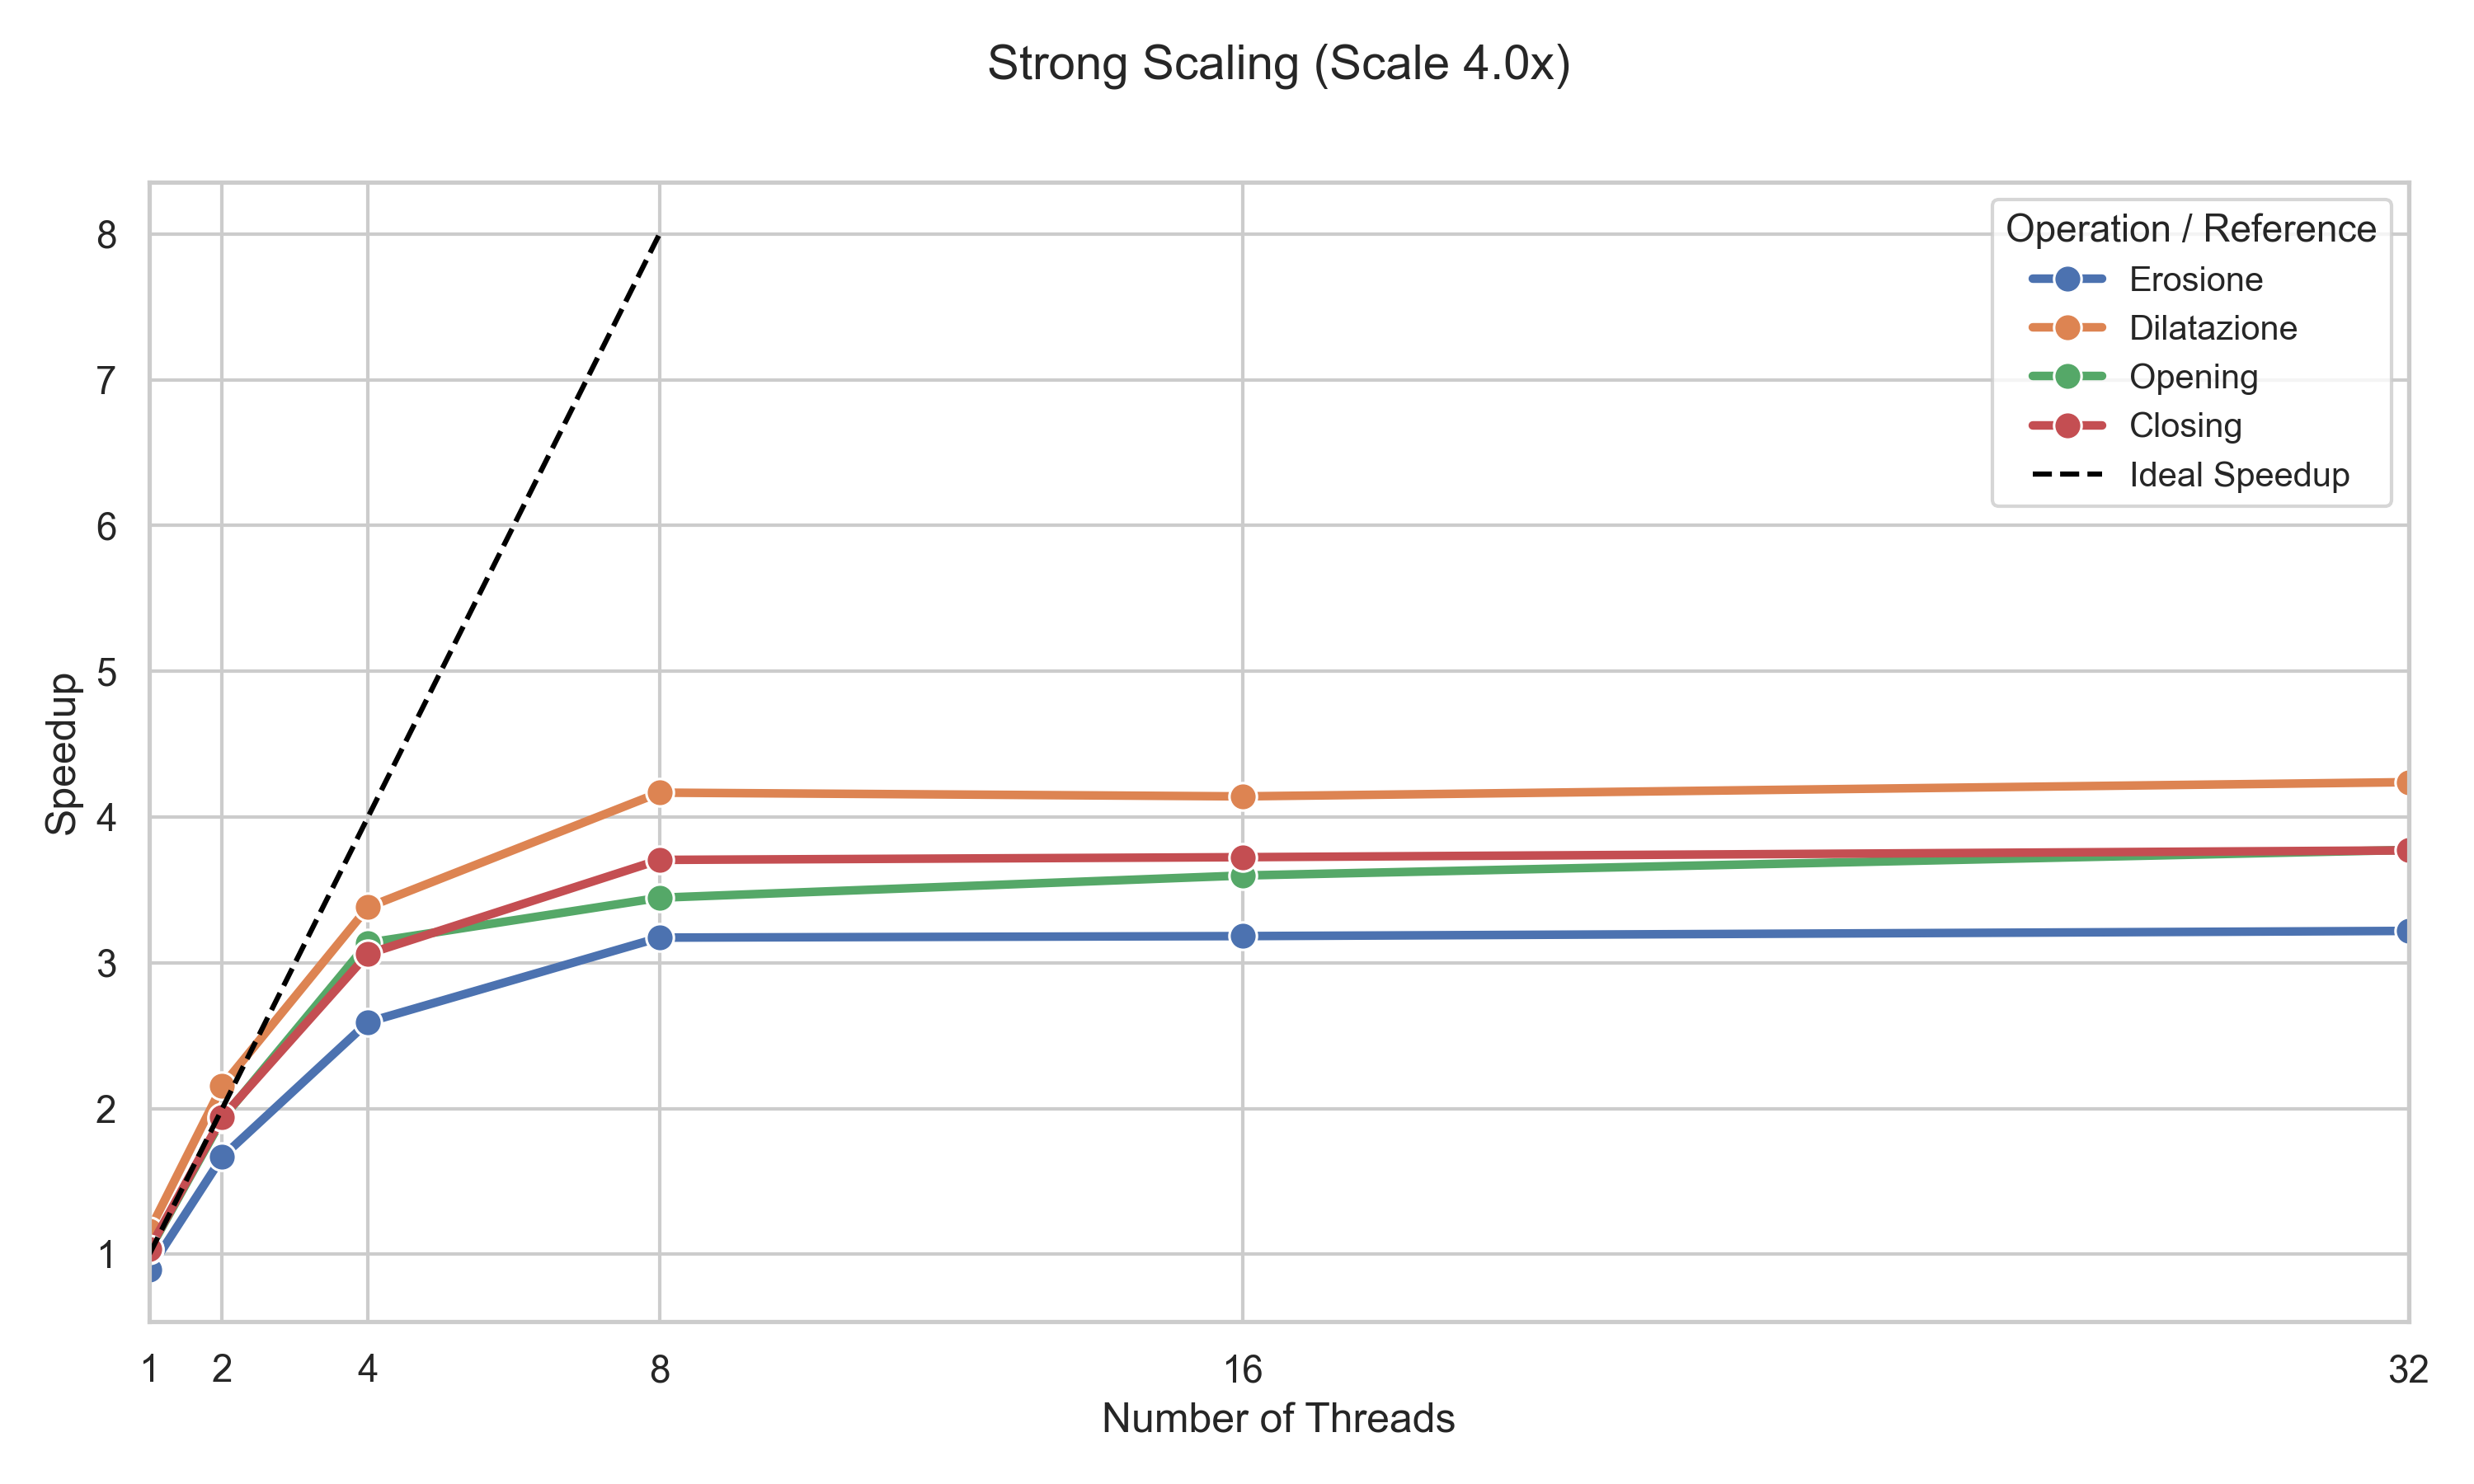
\includegraphics[width=0.85\linewidth]{img/strong_scaling.png}
    \caption{Strong scaling speedup for fixed 4.0x image resolution across different thread counts.}
    \label{fig:strong_scaling}
\end{figure}

\subsubsection{Weak Scaling}
Weak scaling was measured by increasing both
the image resolution (from 1.0x to 4.0x) and the
thread count proportionally (1, 4, and 16 threads).
Ideally, the execution time should remain constant,
yielding an efficiency of 1.0. However, the experimental
data shows a gradual increase in execution time, with
the average parallel efficiency across the four operations
dropping from approximately \textbf{1.0} at 1 thread to
\textbf{0.73} at 4 threads, and collapsing further to
\textbf{0.23} at 16 threads. This behavior confirms that
as the data volume grows, the spatial locality of the
cache hierarchy degrades; the overhead of managing a
lot of threads in a Fork-Join model and the strict RAM
bandwidth limits for large matrices, makes perfect weak
scaling unachievable for this specific memory-bound
workload.

\begin{figure}[htbp]
    \centering
    \begin{minipage}{0.48\textwidth}
        \centering
        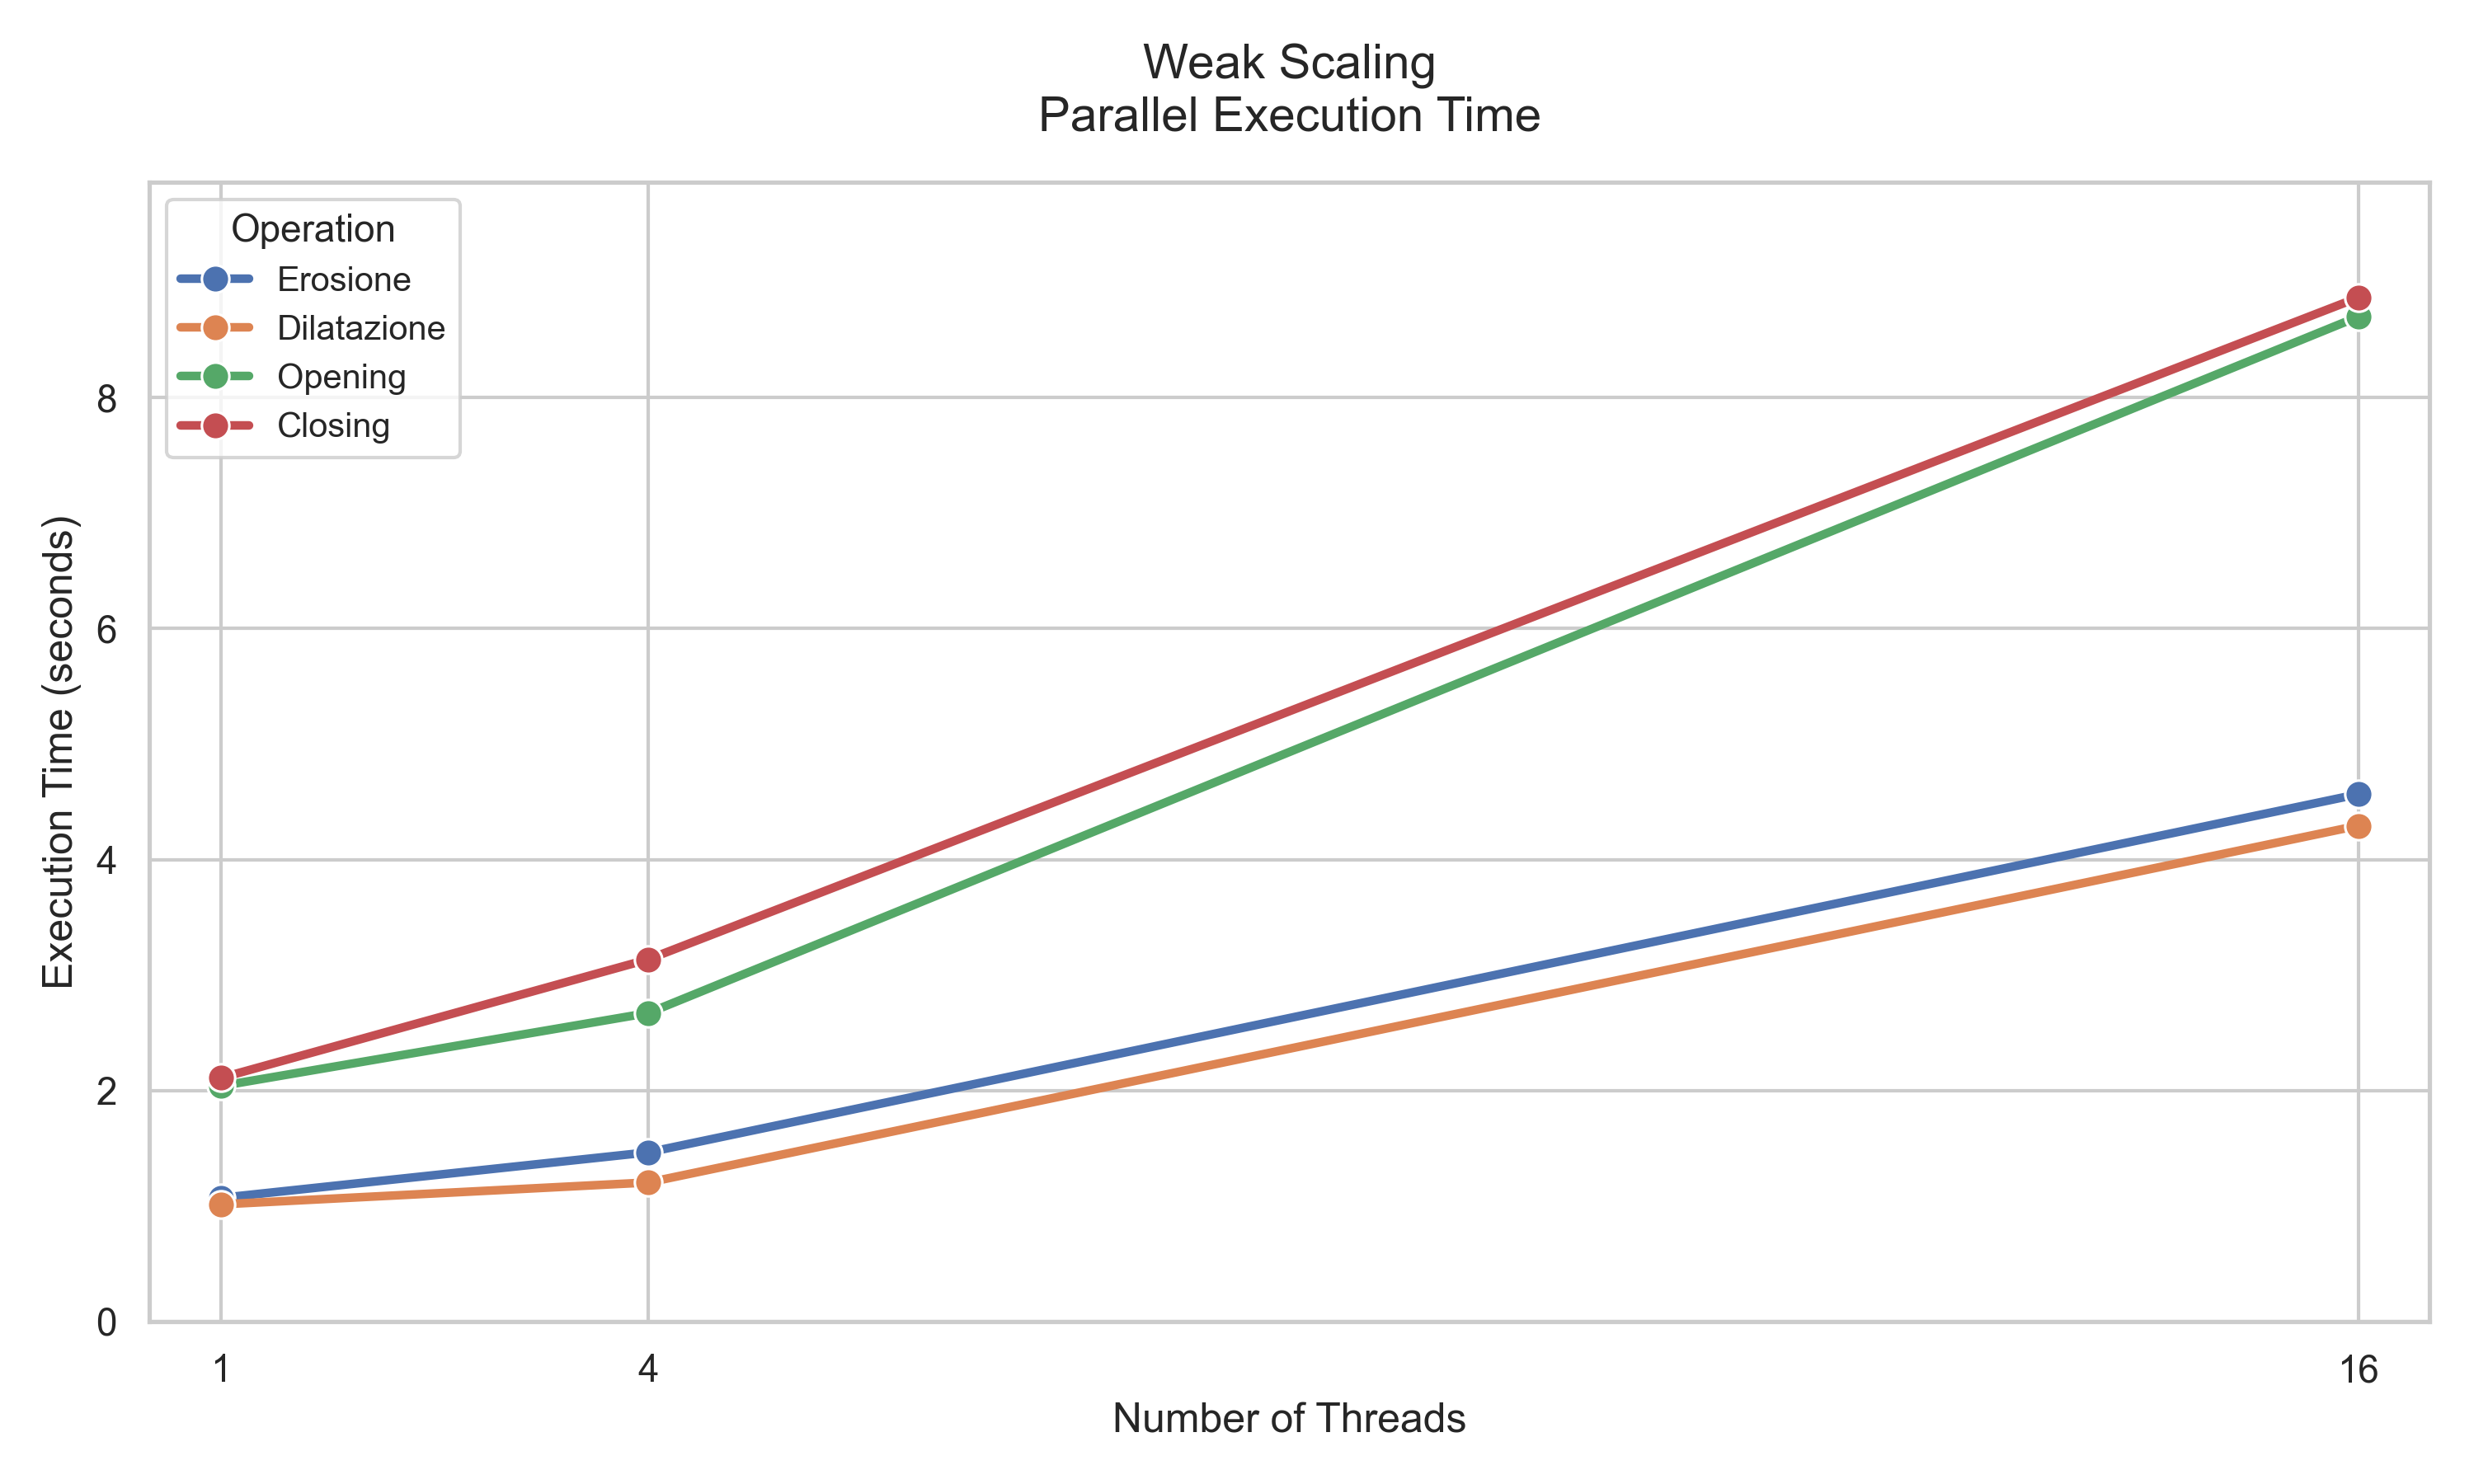
\includegraphics[width=\linewidth]{img/weak_scaling_time.png}
        \caption{Execution time in weak scaling tests.}
        \label{fig:weak_scaling_time}
    \end{minipage}
    \hfill
    \begin{minipage}{0.48\textwidth}
        \centering
        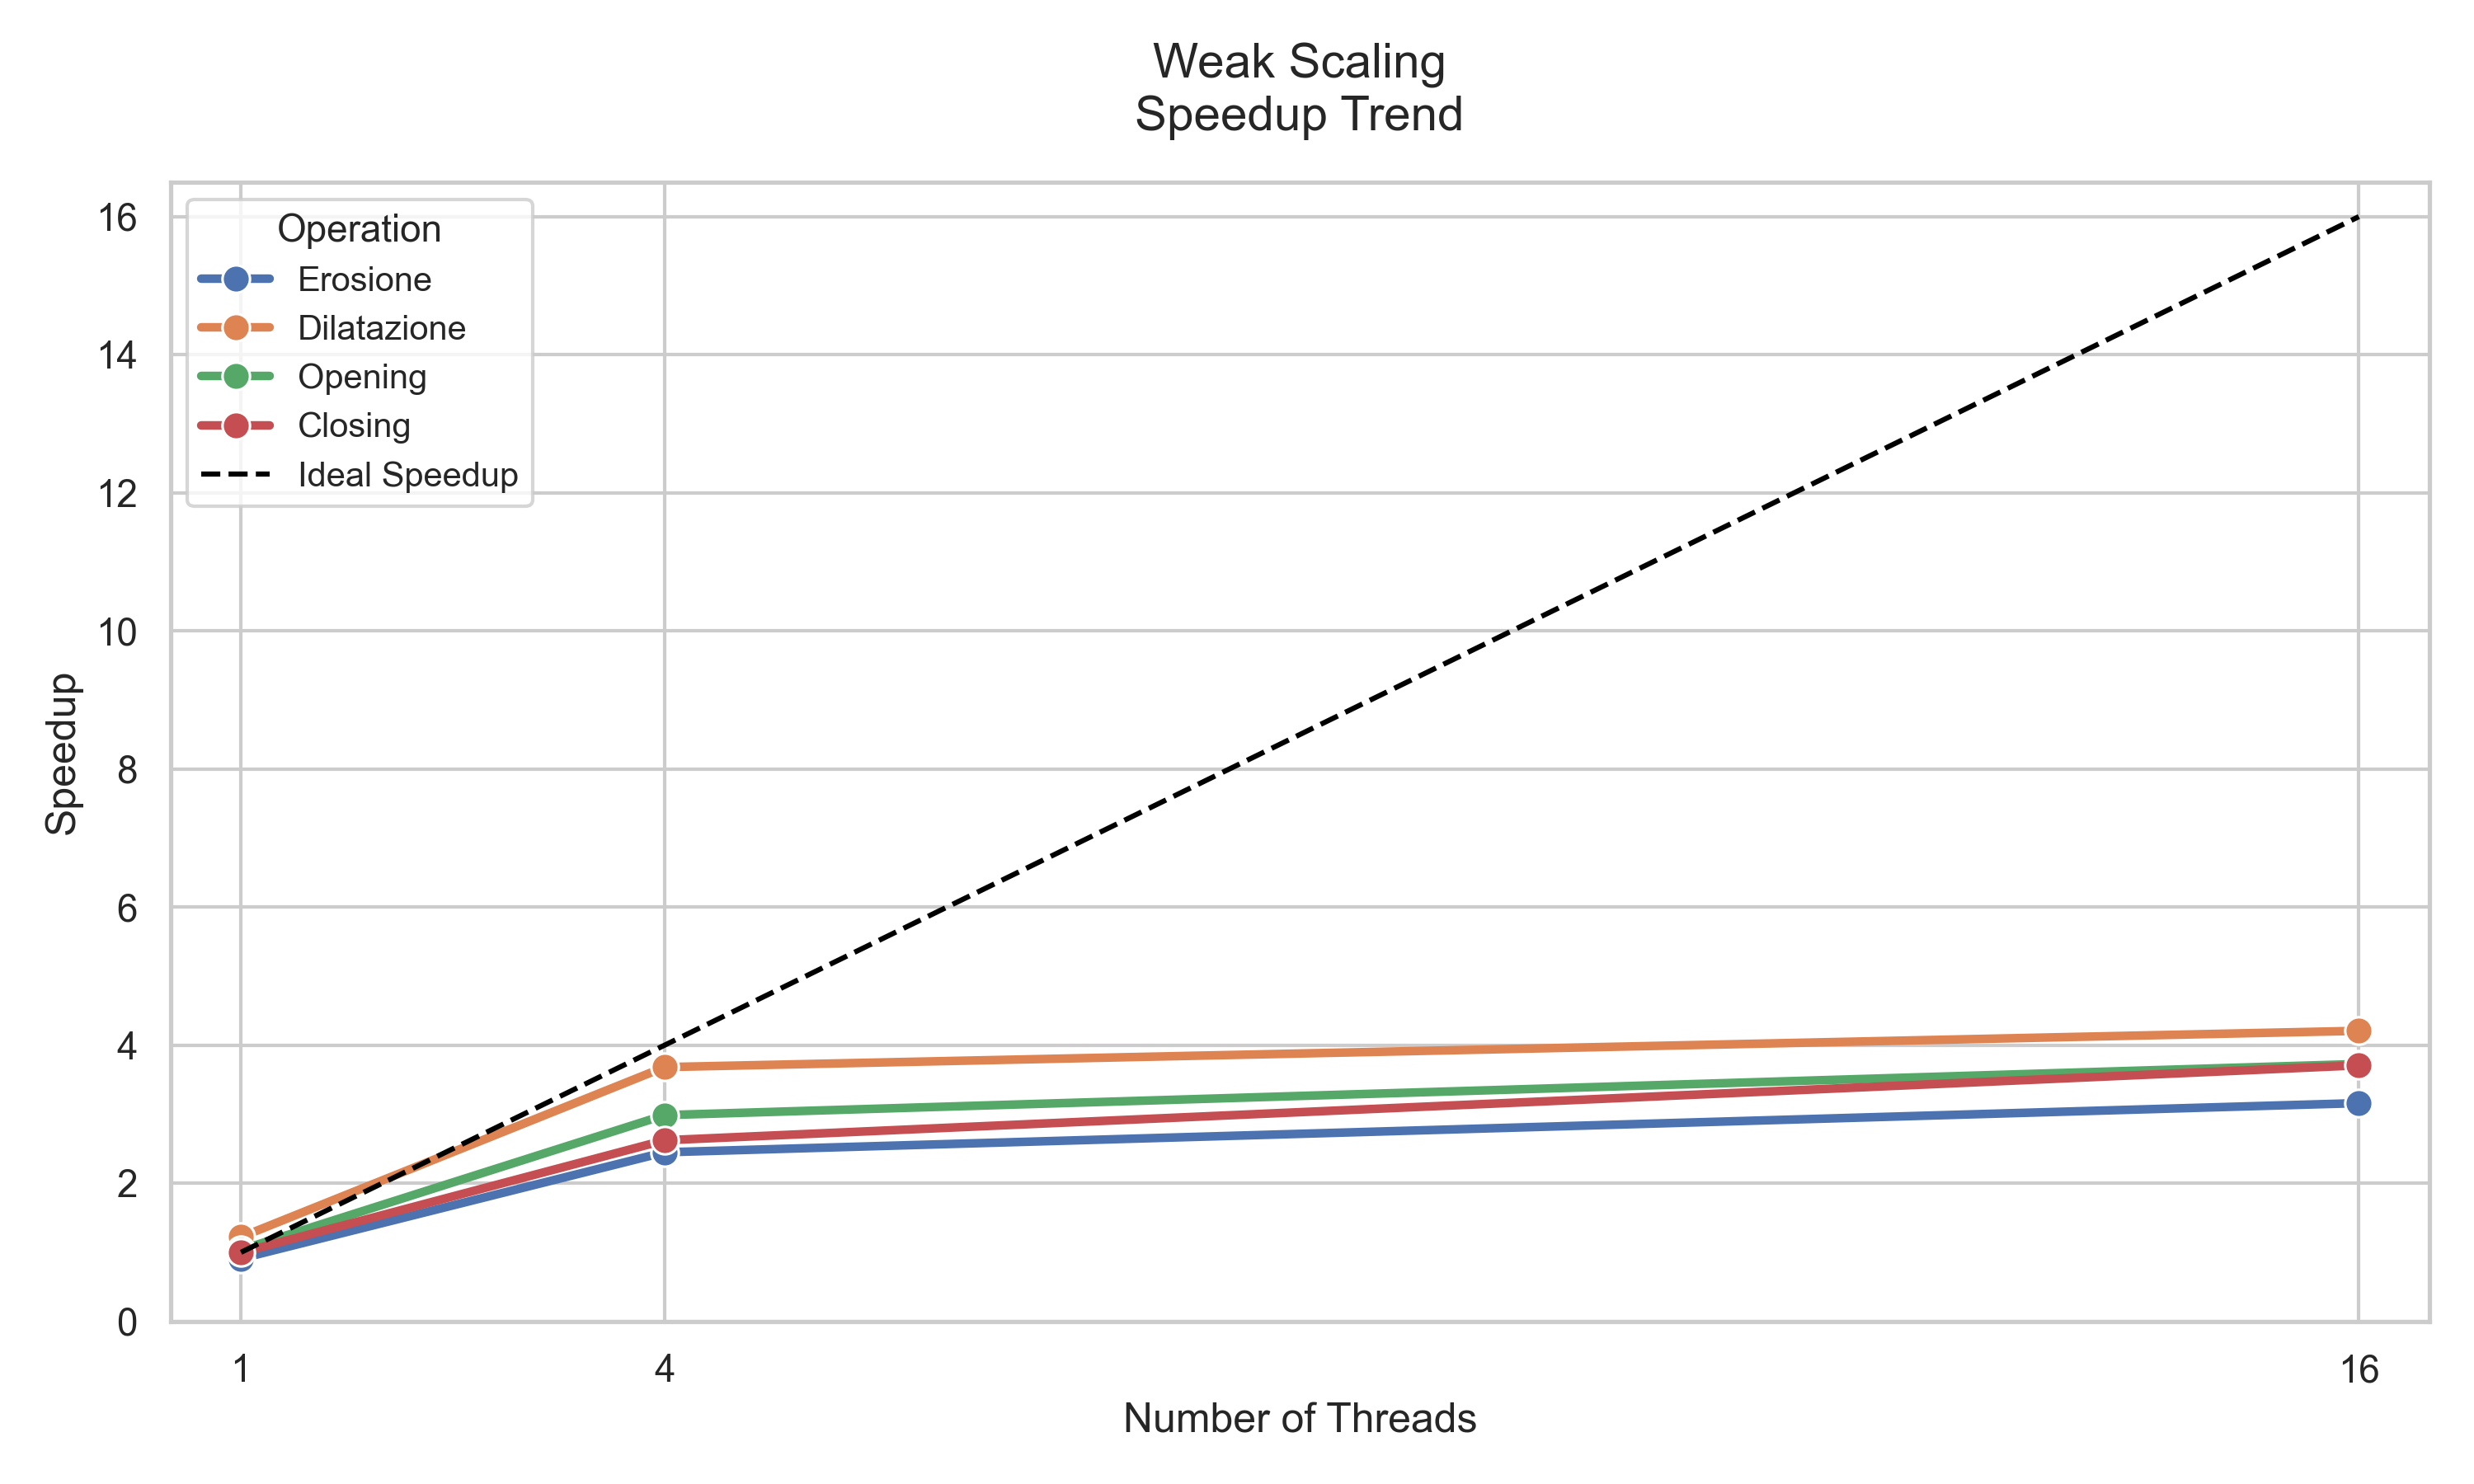
\includegraphics[width=\linewidth]{img/weak_scaling_speedup.png}
        \caption{Parallel efficiency and speedup in weak scaling.}
        \label{fig:weak_scaling_speedup}
    \end{minipage}
\end{figure}
 
\subsection{Impact of Algorithmic Optimization: 2D vs. 1D Separable Kernels}
The transition from a 2D spatial domain stencil to a 1D separable kernel represents the most significant performance gain in the framework. This optimization fundamentally alters the arithmetic complexity, reducing it from $\mathcal{O}(K^2)$ to $\mathcal{O}(2K)$ operations per pixel. 

As shown in the separable speedup plots (Figure \ref{fig:separable_speedup_comparison}) comparing the 2.0x and 4.0x image scales, the performance gain is intrinsically dependent on the kernel size $K$, while also exhibiting a subtle sensitivity to the overall image resolution. For small kernels ($K=3$), the speedup is marginal across both resolutions, ranging between approximately \textbf{1.2x} and \textbf{1.7x}. At this scale, the reduction of mathematical operations is minimal and is nearly offset by the software overhead of executing two separate memory passes (horizontal then vertical) and allocating intermediate buffers. 

On the other hand, for large kernels ($K=15$), the speedup scales dramatically. At the 2.0x scale, performance reaches peaks of \textbf{13.4x} for Dilation and \textbf{6.8x} for Erosion. When increasing the resolution to 4.0x, the peaks remain exceptional (\textbf{11.9x} for Dilation and \textbf{6.6x} for Erosion) but slightly lower compared to the 2.0x scenario. This increase in speedup confirms that for large structuring elements, bypassing over 200 redundant operations per pixel overwhelmingly compensates for the algorithmic overhead. 

A noteworthy observation is the consistent speedup asymmetry between
Dilation and Erosion: for medium and large kernel sizes ($K \geq 7$),
Dilation systematically achieves approximately twice the speedup of
Erosion across both resolutions, an asymmetry that narrows 
at $K=3$ (where the ratio drops to roughly $1.3\times$). Inspecting 
the raw timing data reveals that this asymmetry originates not from a faster 
separable execution, but from a slower 2D parallel baseline for Dilation. 
At $K=15$ with 4 threads, the 2D baseline for Dilation is already significantly 
slower than Erosion at both tested resolutions (30.8s vs. 26.3s at scale 2.0x, 
and 121.5s vs. 88.8s at scale 4.0x), while their separable execution times are 
comparable and even reversed in favor of Dilation (2.29s vs. 3.87s at scale 2.0x, 
and 10.2s vs. 13.5s at scale 4.0x). The speedup gap is therefore a direct 
consequence of Dilation having a larger numerator in the speedup ratio, not a 
smaller denominator.

A plausible, though unverified, hypothesis for this behavioral asymmetry in the 
2D baseline lies in how the two accumulators interact with the inner loop structure. 
The Erosion accumulator (\lstinline|min_val = 255|) decreases monotonically: it 
converges rapidly to a stable low value, allowing the compiler to potentially 
exploit this pattern during loop unrolling or auto-vectorization. In contrast, the 
Dilation accumulator (\lstinline|max_val = 0|) rises sharply on the first 
encountered neighbor and then stalls at a high threshold, forcing the CPU to 
evaluate comparisons that rarely produce updates against an already near-maximum 
value. This subtle difference in convergence behavior may produce a less optimized 
inner loop at the assembly level for Dilation, inflating its 2D baseline cost. 
A definitive confirmation would require dedicated hardware performance counter 
profiling (e.g., via \texttt{perf} or \texttt{VTune}).

\begin{figure}[htbp]
    \centering
    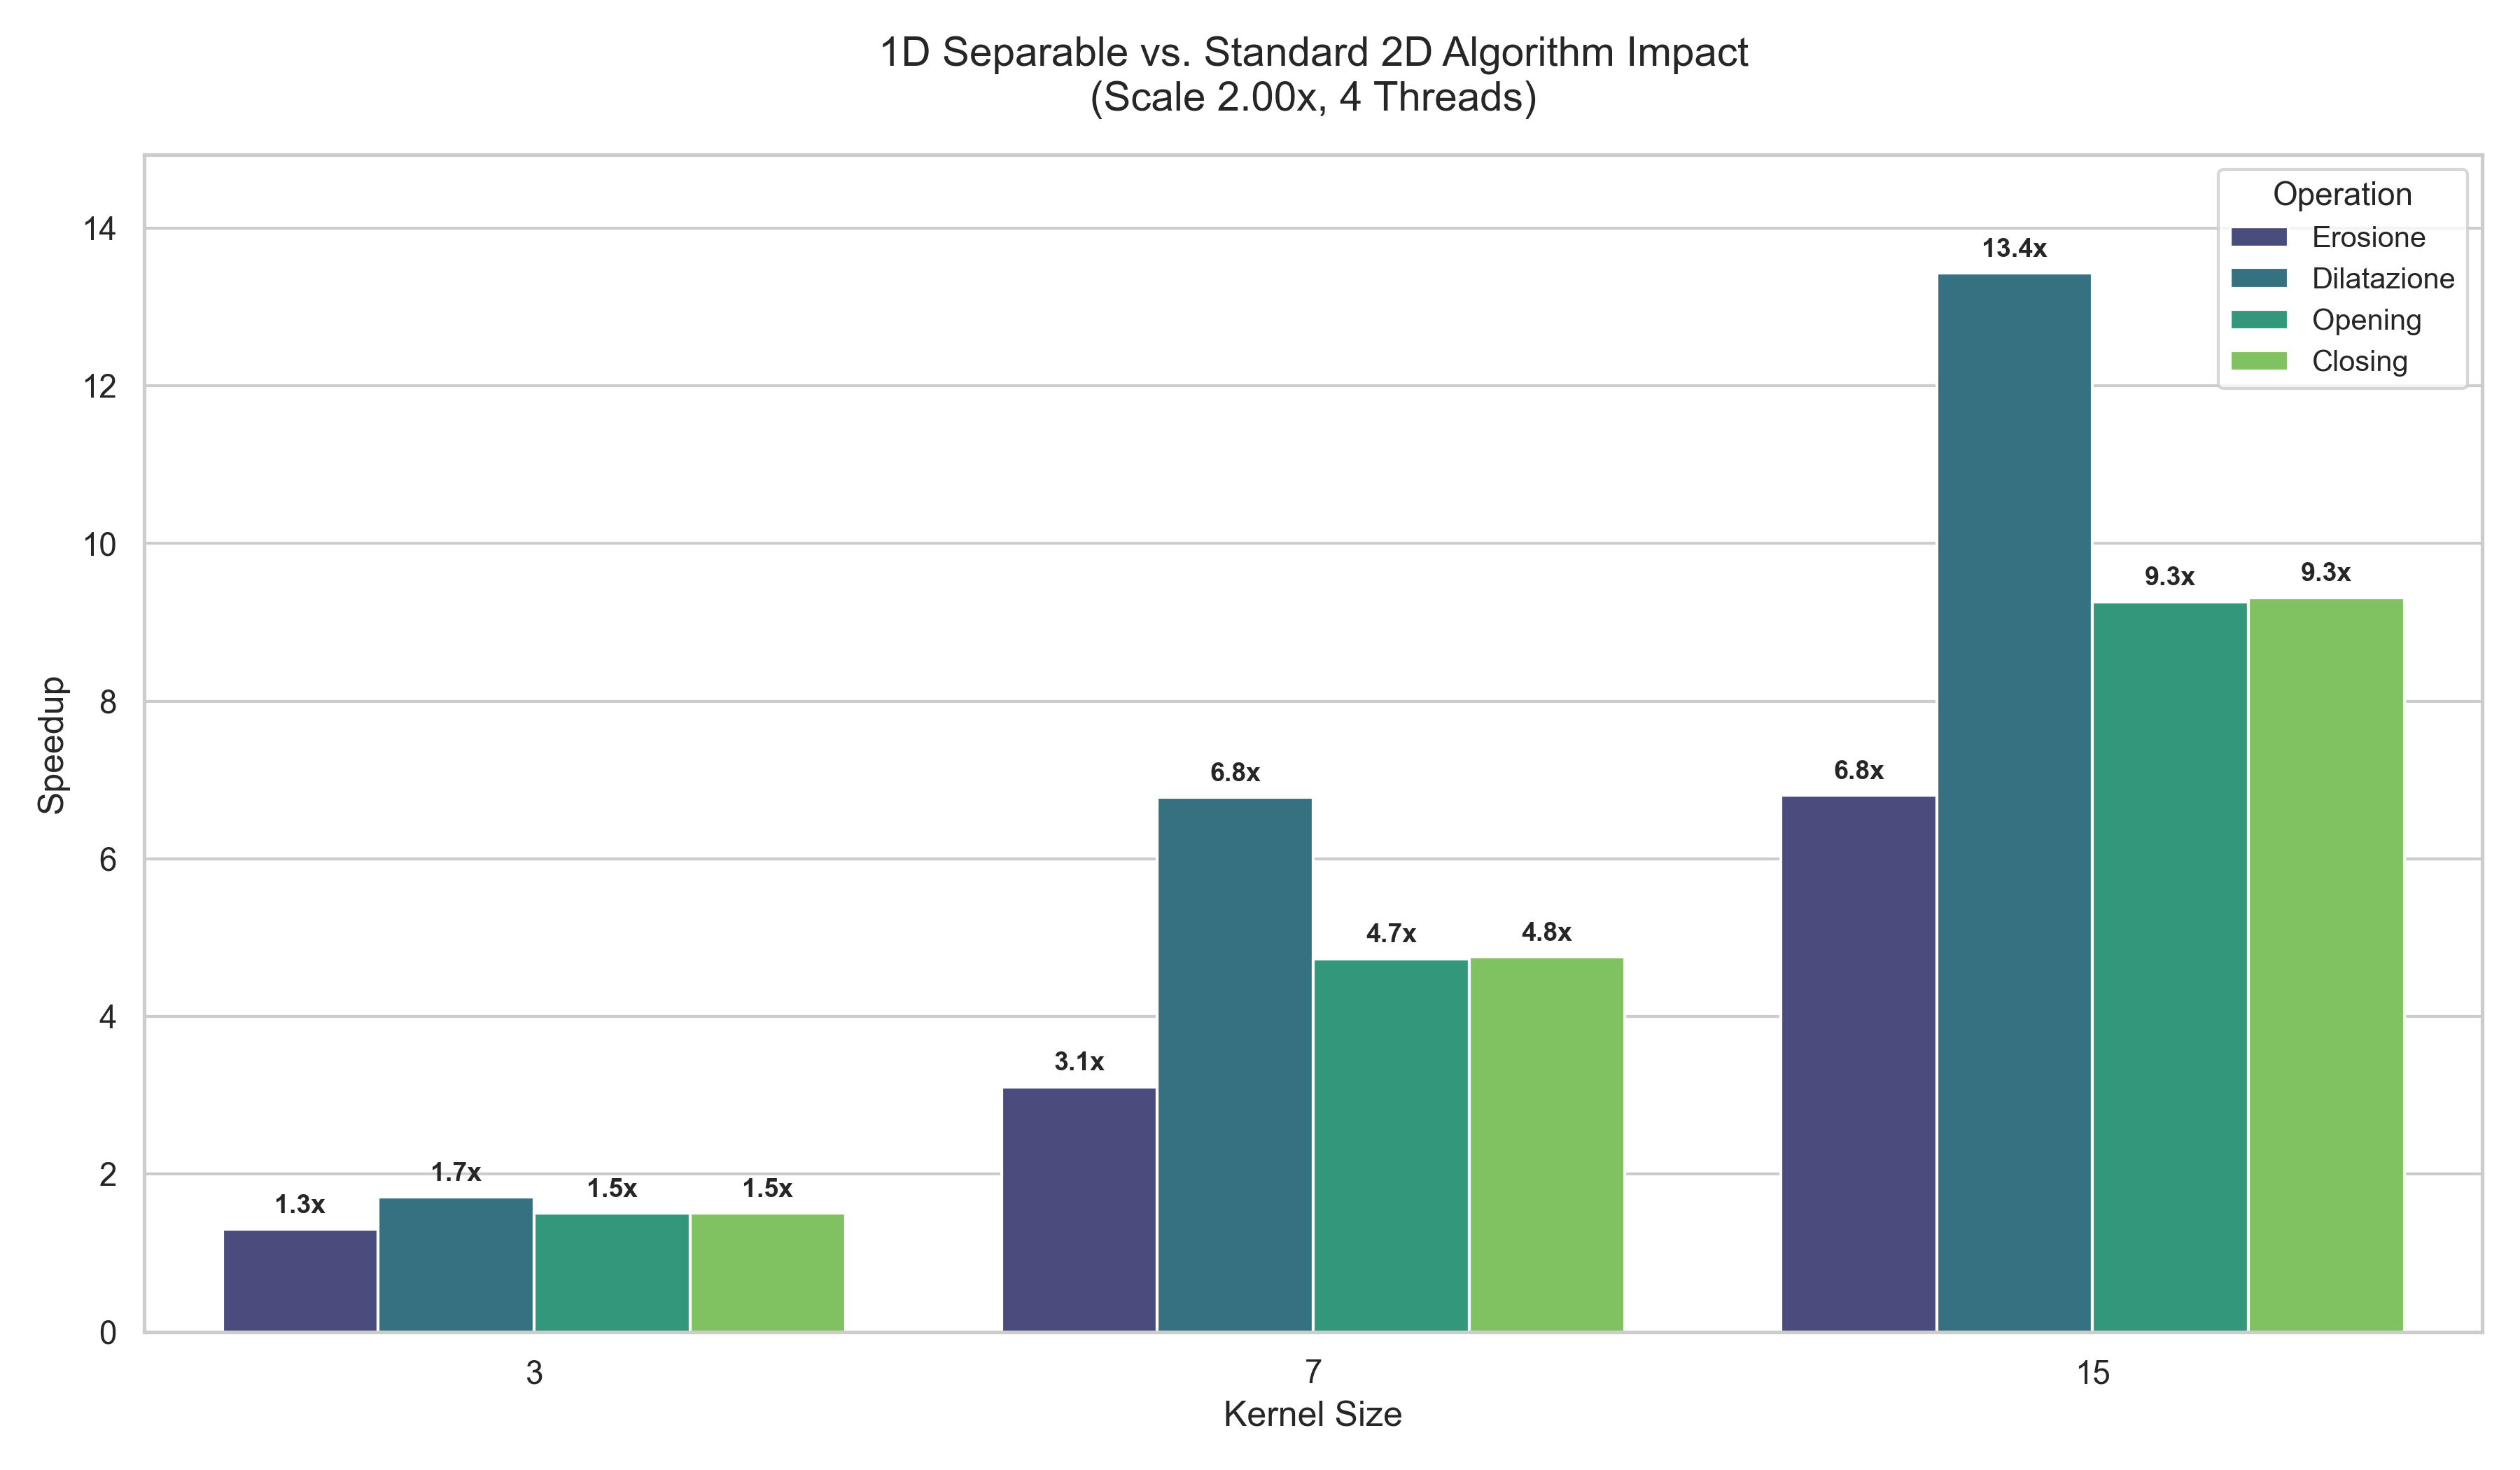
\includegraphics[width=\linewidth]{img/separable_speedup_scale_2.0x.png}
    \caption*{a) Scale 2.0x}
    
    \vspace{0.5cm} % Spazio verticale tra la prima e la seconda immagine
    
    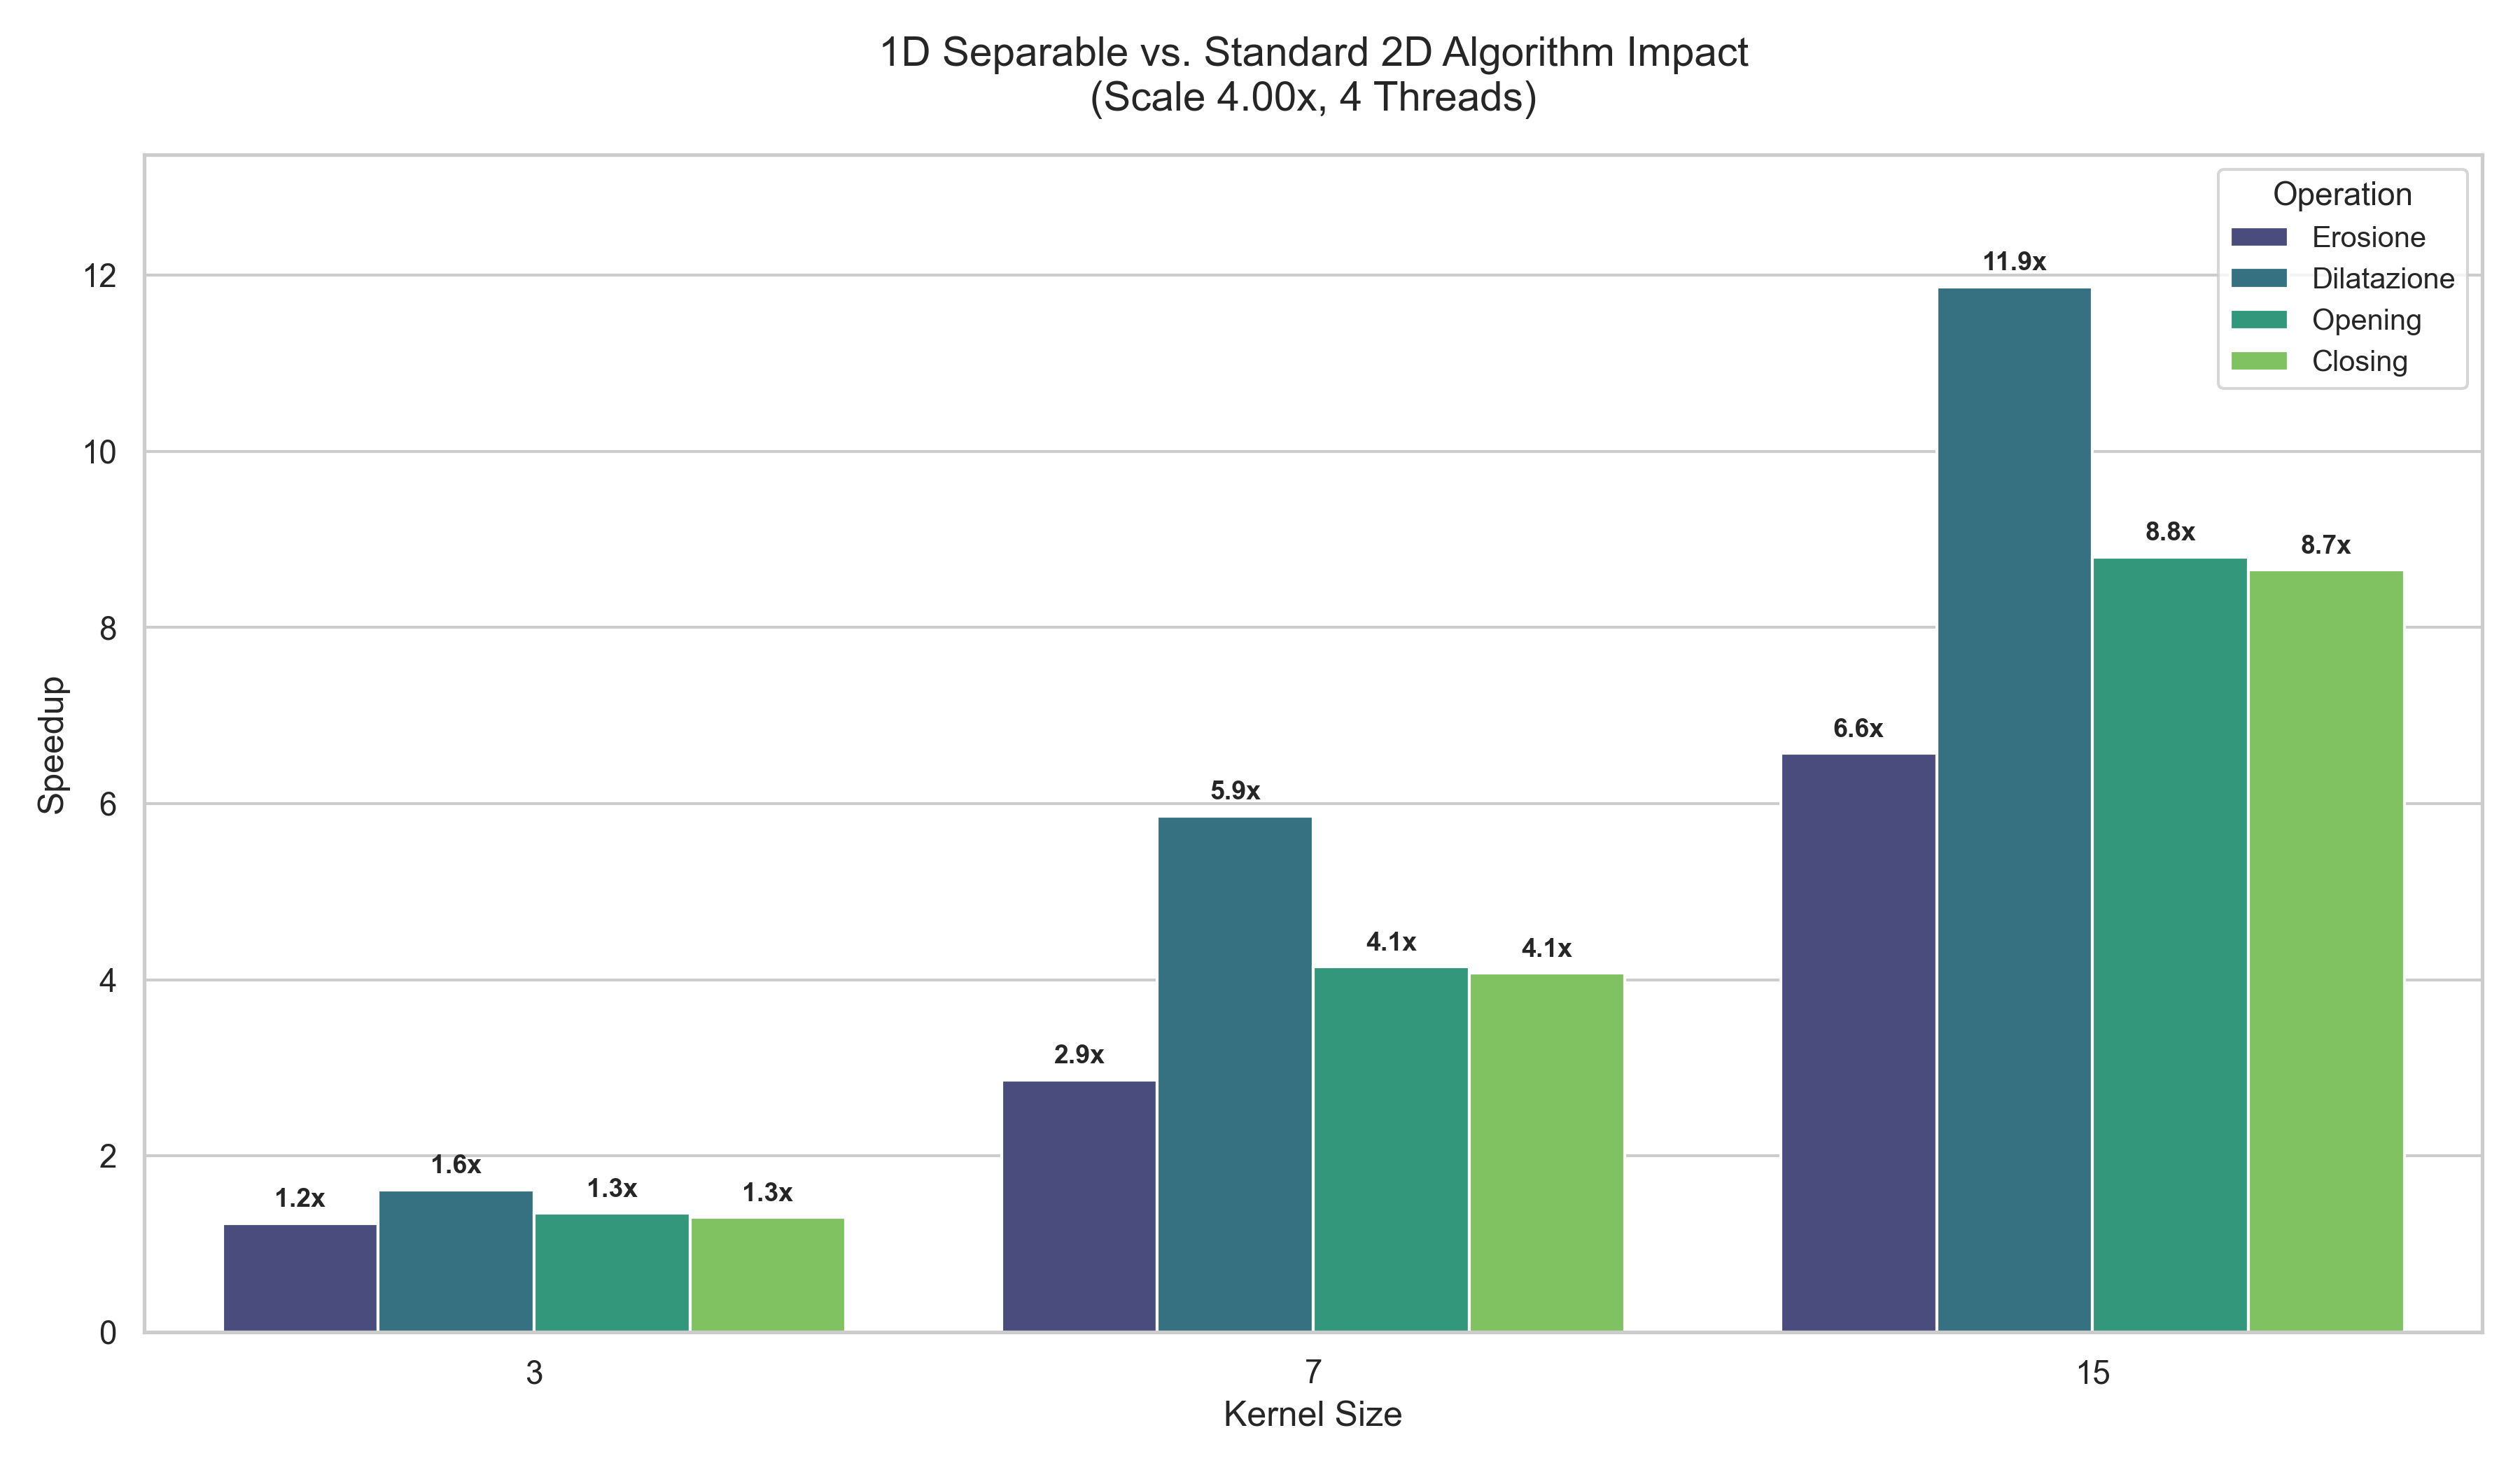
\includegraphics[width=\linewidth]{img/separable_speedup_scale_4.0x.png}
    \caption*{b) Scale 4.0x}
    
    \caption{Comparison of 1D Separable Kernels speedup against the 2D baseline at 2.0x and 4.0x image scales (4 Threads).}
    \label{fig:separable_speedup_comparison}
\end{figure}

\subsection{Pipeline Efficiency for Composite Operations}
Composite operations such as Opening and Closing traditionally suffer from a 
"cascading bottleneck" (as illustrated in a previous section): the first morphological step must complete entirely 
before the second can begin, forcing a full intermediate buffer to be written to 
and read back from main memory. The custom Producer-Consumer pipeline addresses 
this by overlapping the two stages at a fixed granularity of 32-row chunks: 
producer threads apply the first morphological operation row by row within their 
assigned chunks, and upon completion atomically mark each chunk as ready via a 
\lstinline|chunk_ready| flag. Consumer threads do not wait for the entire image 
to be processed; instead, they compute the exact range of chunks strictly required 
by the kernel radius for their assigned output block and spin-wait exclusively on 
those, minimizing unnecessary synchronization.

The experimental results confirm the validity of this architectural choice.
As shown in Figure~\ref{fig:pipeline_speedup}, the 
pipeline consistently outperforms the standard parallel baseline, achieving speedups 
ranging from approximately \textbf{1.2x} to \textbf{1.5x} depending on the image 
resolution and thread count. However, the speedup exhibits a 
monotonically decreasing trend as the number of threads increases: at 2 
threads the gain peaks at roughly \textbf{1.41x} (scale 1.0x) and \textbf{1.52x} 
(scale 2.0x), while at 8 threads it degrades to approximately \textbf{1.20x} and 
\textbf{1.35x} respectively.

This degradation could be a consequence of the pipeline design. With 
only 2 threads, the producer-consumer split is perfectly balanced: one thread 
generates chunks while the other immediately consumes them, maximizing temporal 
cache locality and keeping intermediate data hot in the L1/L2 cache. As the thread 
count increases, the total thread pool is still divided equally between producers 
and consumers, but the spin-wait synchronization overhead grows 
proportionally: even though each consumer polls only the strictly necessary chunks, 
the number of atomic read operations on \lstinline|chunk_ready| accumulates across 
the growing number of consumer threads, introducing a considerable serialization 
cost. With more threads competing for the same shared 
\lstinline|temp_eroded| buffer, cache coherence traffic intensifies, partially 
undermining the locality benefits that motivate the pipeline approach in the 
first place.

\begin{figure}[htbp]
    \centering
    \begin{minipage}{0.48\textwidth}
        \centering
        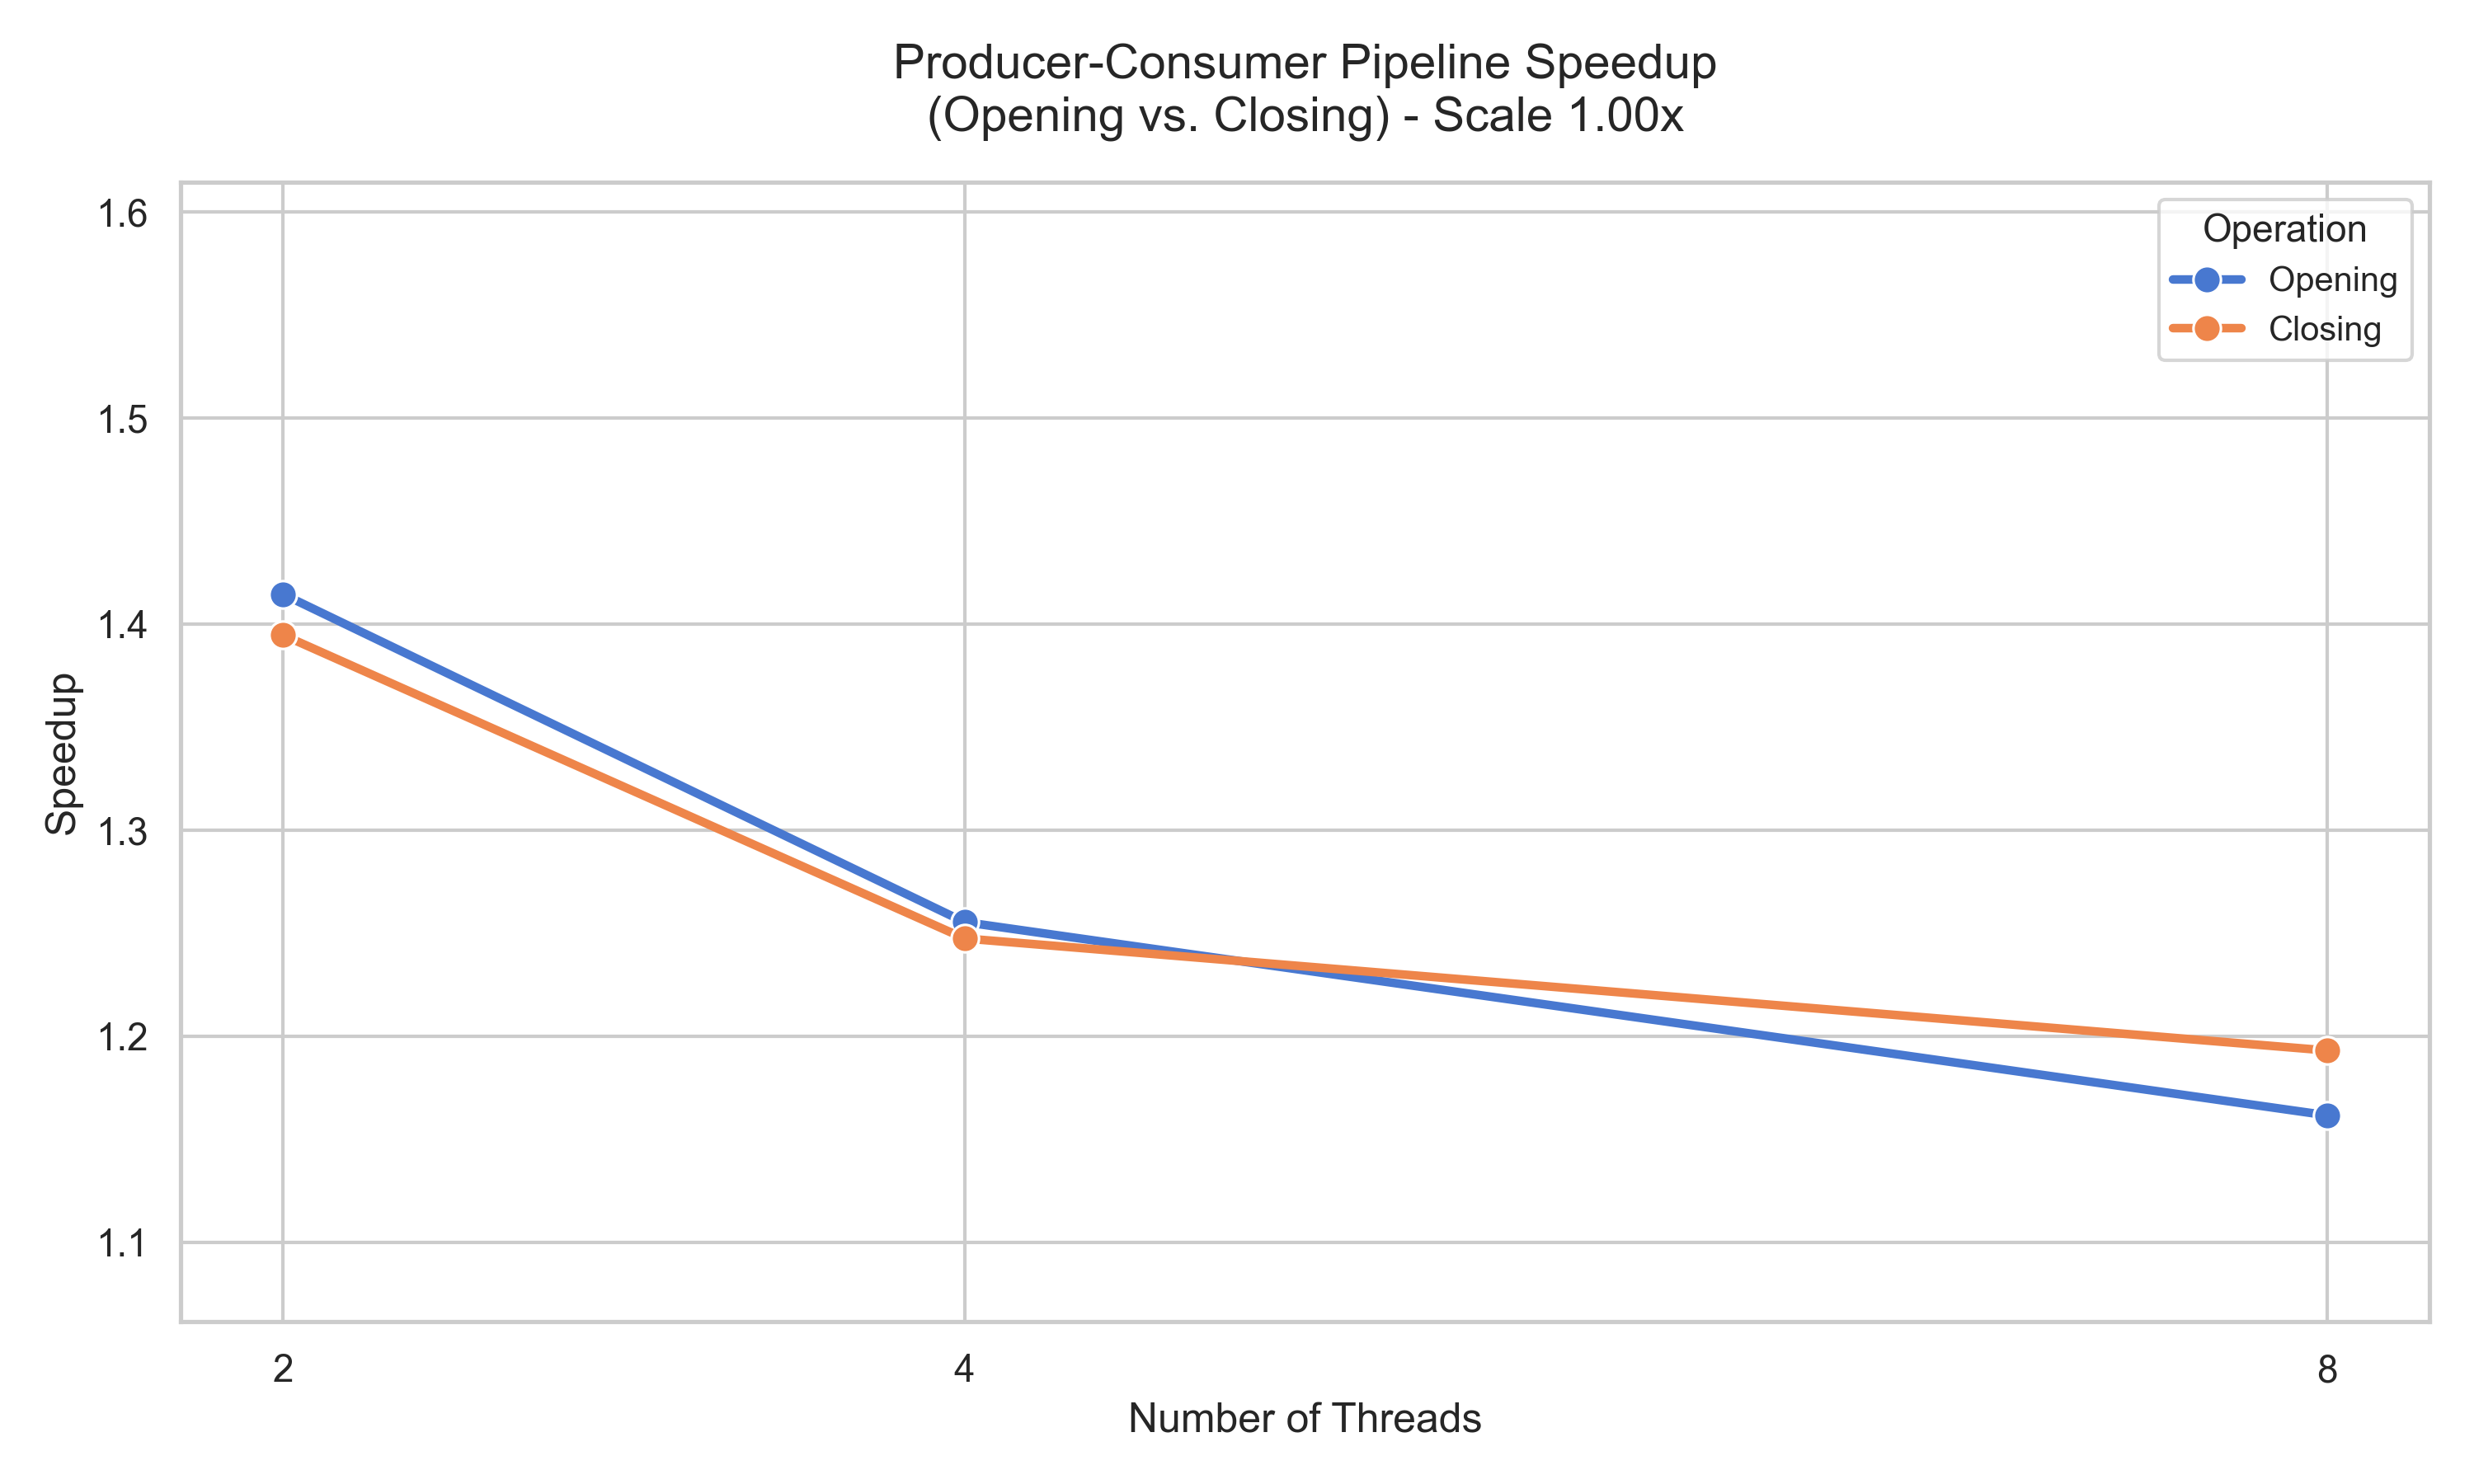
\includegraphics[width=\linewidth]{img/pipeline_speedup_scale_1.0x.png}
        \caption*{a) Scale 1.0x}
    \end{minipage}\hfill
    \begin{minipage}{0.48\textwidth}
        \centering
        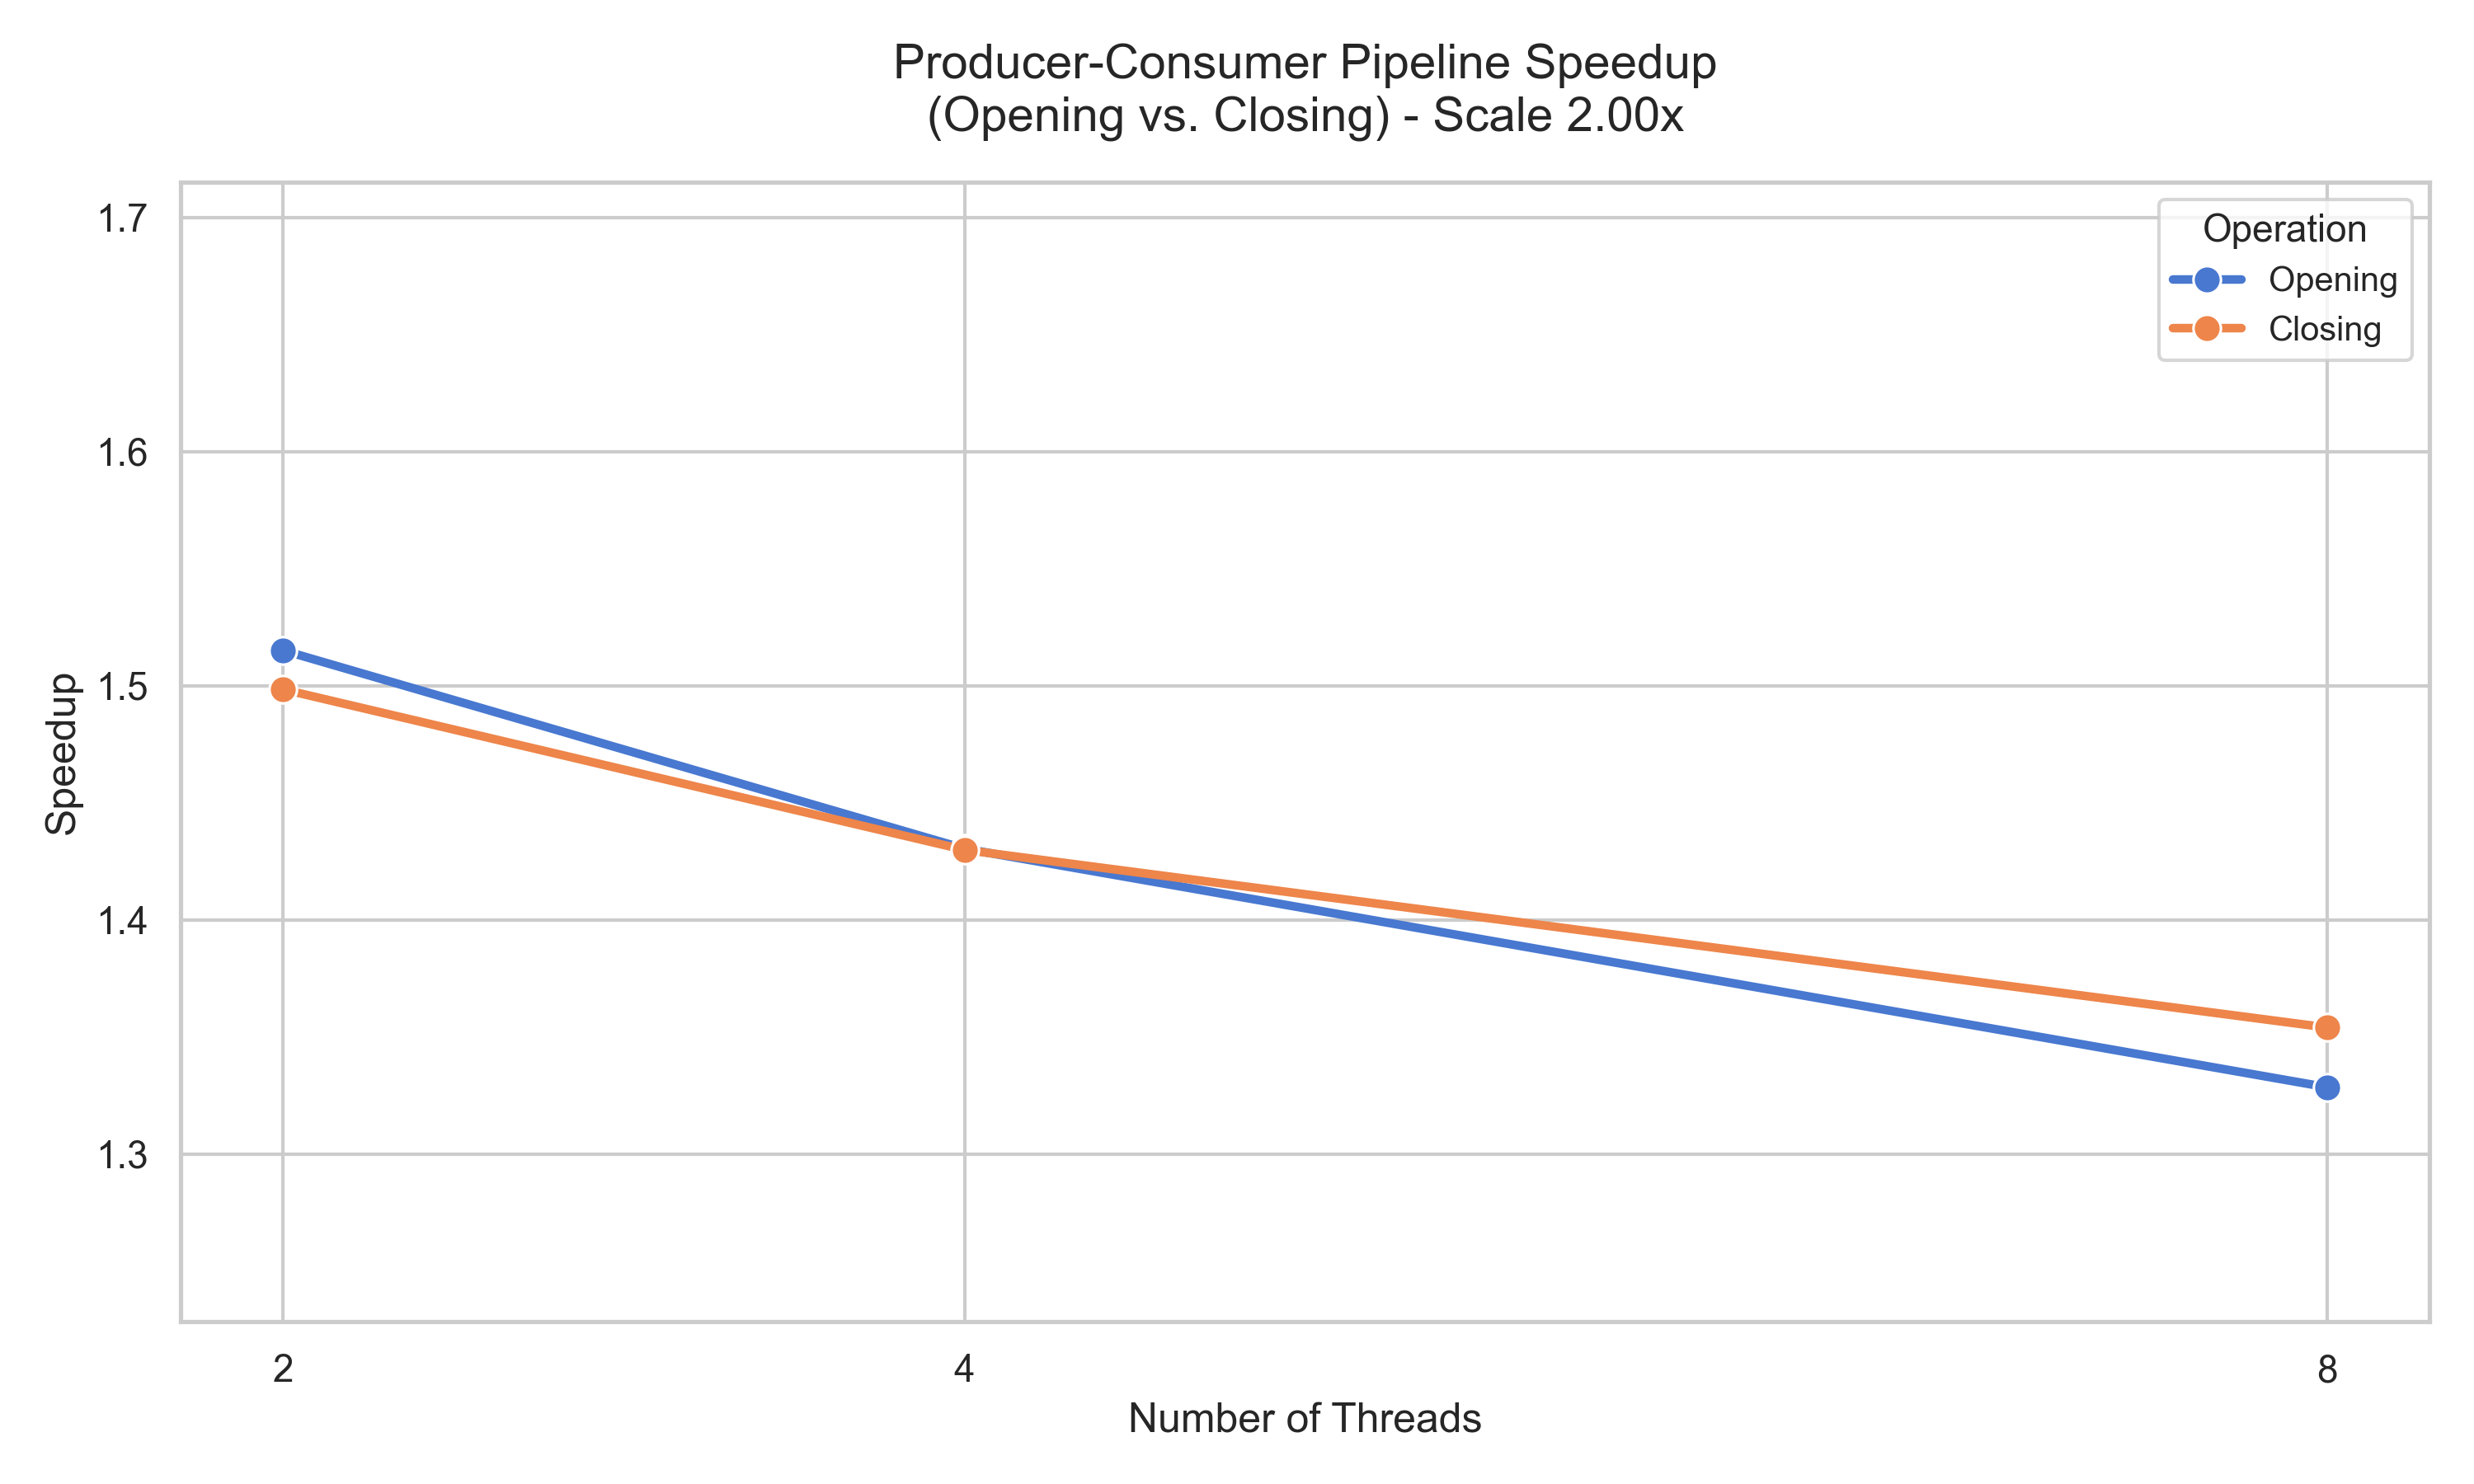
\includegraphics[width=\linewidth]{img/pipeline_speedup_scale_2.0x.png}
        \caption*{b) Scale 2.0x}
    \end{minipage}
    \caption{Producer-Consumer pipeline speedup over the standard parallel baseline 
    for Opening and Closing operations, at scale 1.0x and 2.0x across increasing 
    thread counts.}
    \label{fig:pipeline_speedup}
\end{figure}

\subsection{Optimal Parallel vs. Sequential Baseline}
To quantify the absolute performance ceiling of the framework, the fully optimized 
parallel implementation was benchmarked directly against the naive sequential 2D 
baseline across all three resolutions (1.0x, 2.0x, 4.0x) and kernel sizes 
($K \in \{3, 7, 15\}$), using 4 threads. The optimal configuration combines three 
synergistic design choices: 1D separable kernels to reduce per-pixel 
complexity from $\mathcal{O}(K^2)$ to $\mathcal{O}(2K)$, \texttt{collapse(2)} 
to maximize the parallel iteration space, and dynamic scheduling to 
mitigate OS jitter and thread load imbalance.

The Figure~\ref{fig:optimal_speedup} reveals two key 
properties of the optimized framework. First, the speedup scales 
quasi-linearly with the kernel size: from approximately \textbf{2x} at 
$K=3$, to \textbf{8x} at $K=7$, up to a peak of \textbf{22x} at $K=15$. This 
linearity is the direct empirical signature of the complexity reduction: 
mathematically, the theoretical algorithmic speedup is proportional to the 
ratio of their operations, $\frac{K^2}{2K} = \frac{K}{2}$, resulting in a 
linear growth that compounds with the thread-level parallelism provided by OpenMP.

Second, the three resolution curves (1.0x, 2.0x, 4.0x) are nearly 
indistinguishable across all kernel sizes. This resolution-invariance confirms that the dominant factor governing 
speedup is the algorithmic complexity reduction rather than 
parallelization efficiency or memory bandwidth: the separable decomposition 
eliminates the same proportion of redundant operations regardless of image size, 
making the framework robust and predictably scalable across different input 
resolutions.

\begin{figure}[htbp]
    \centering
    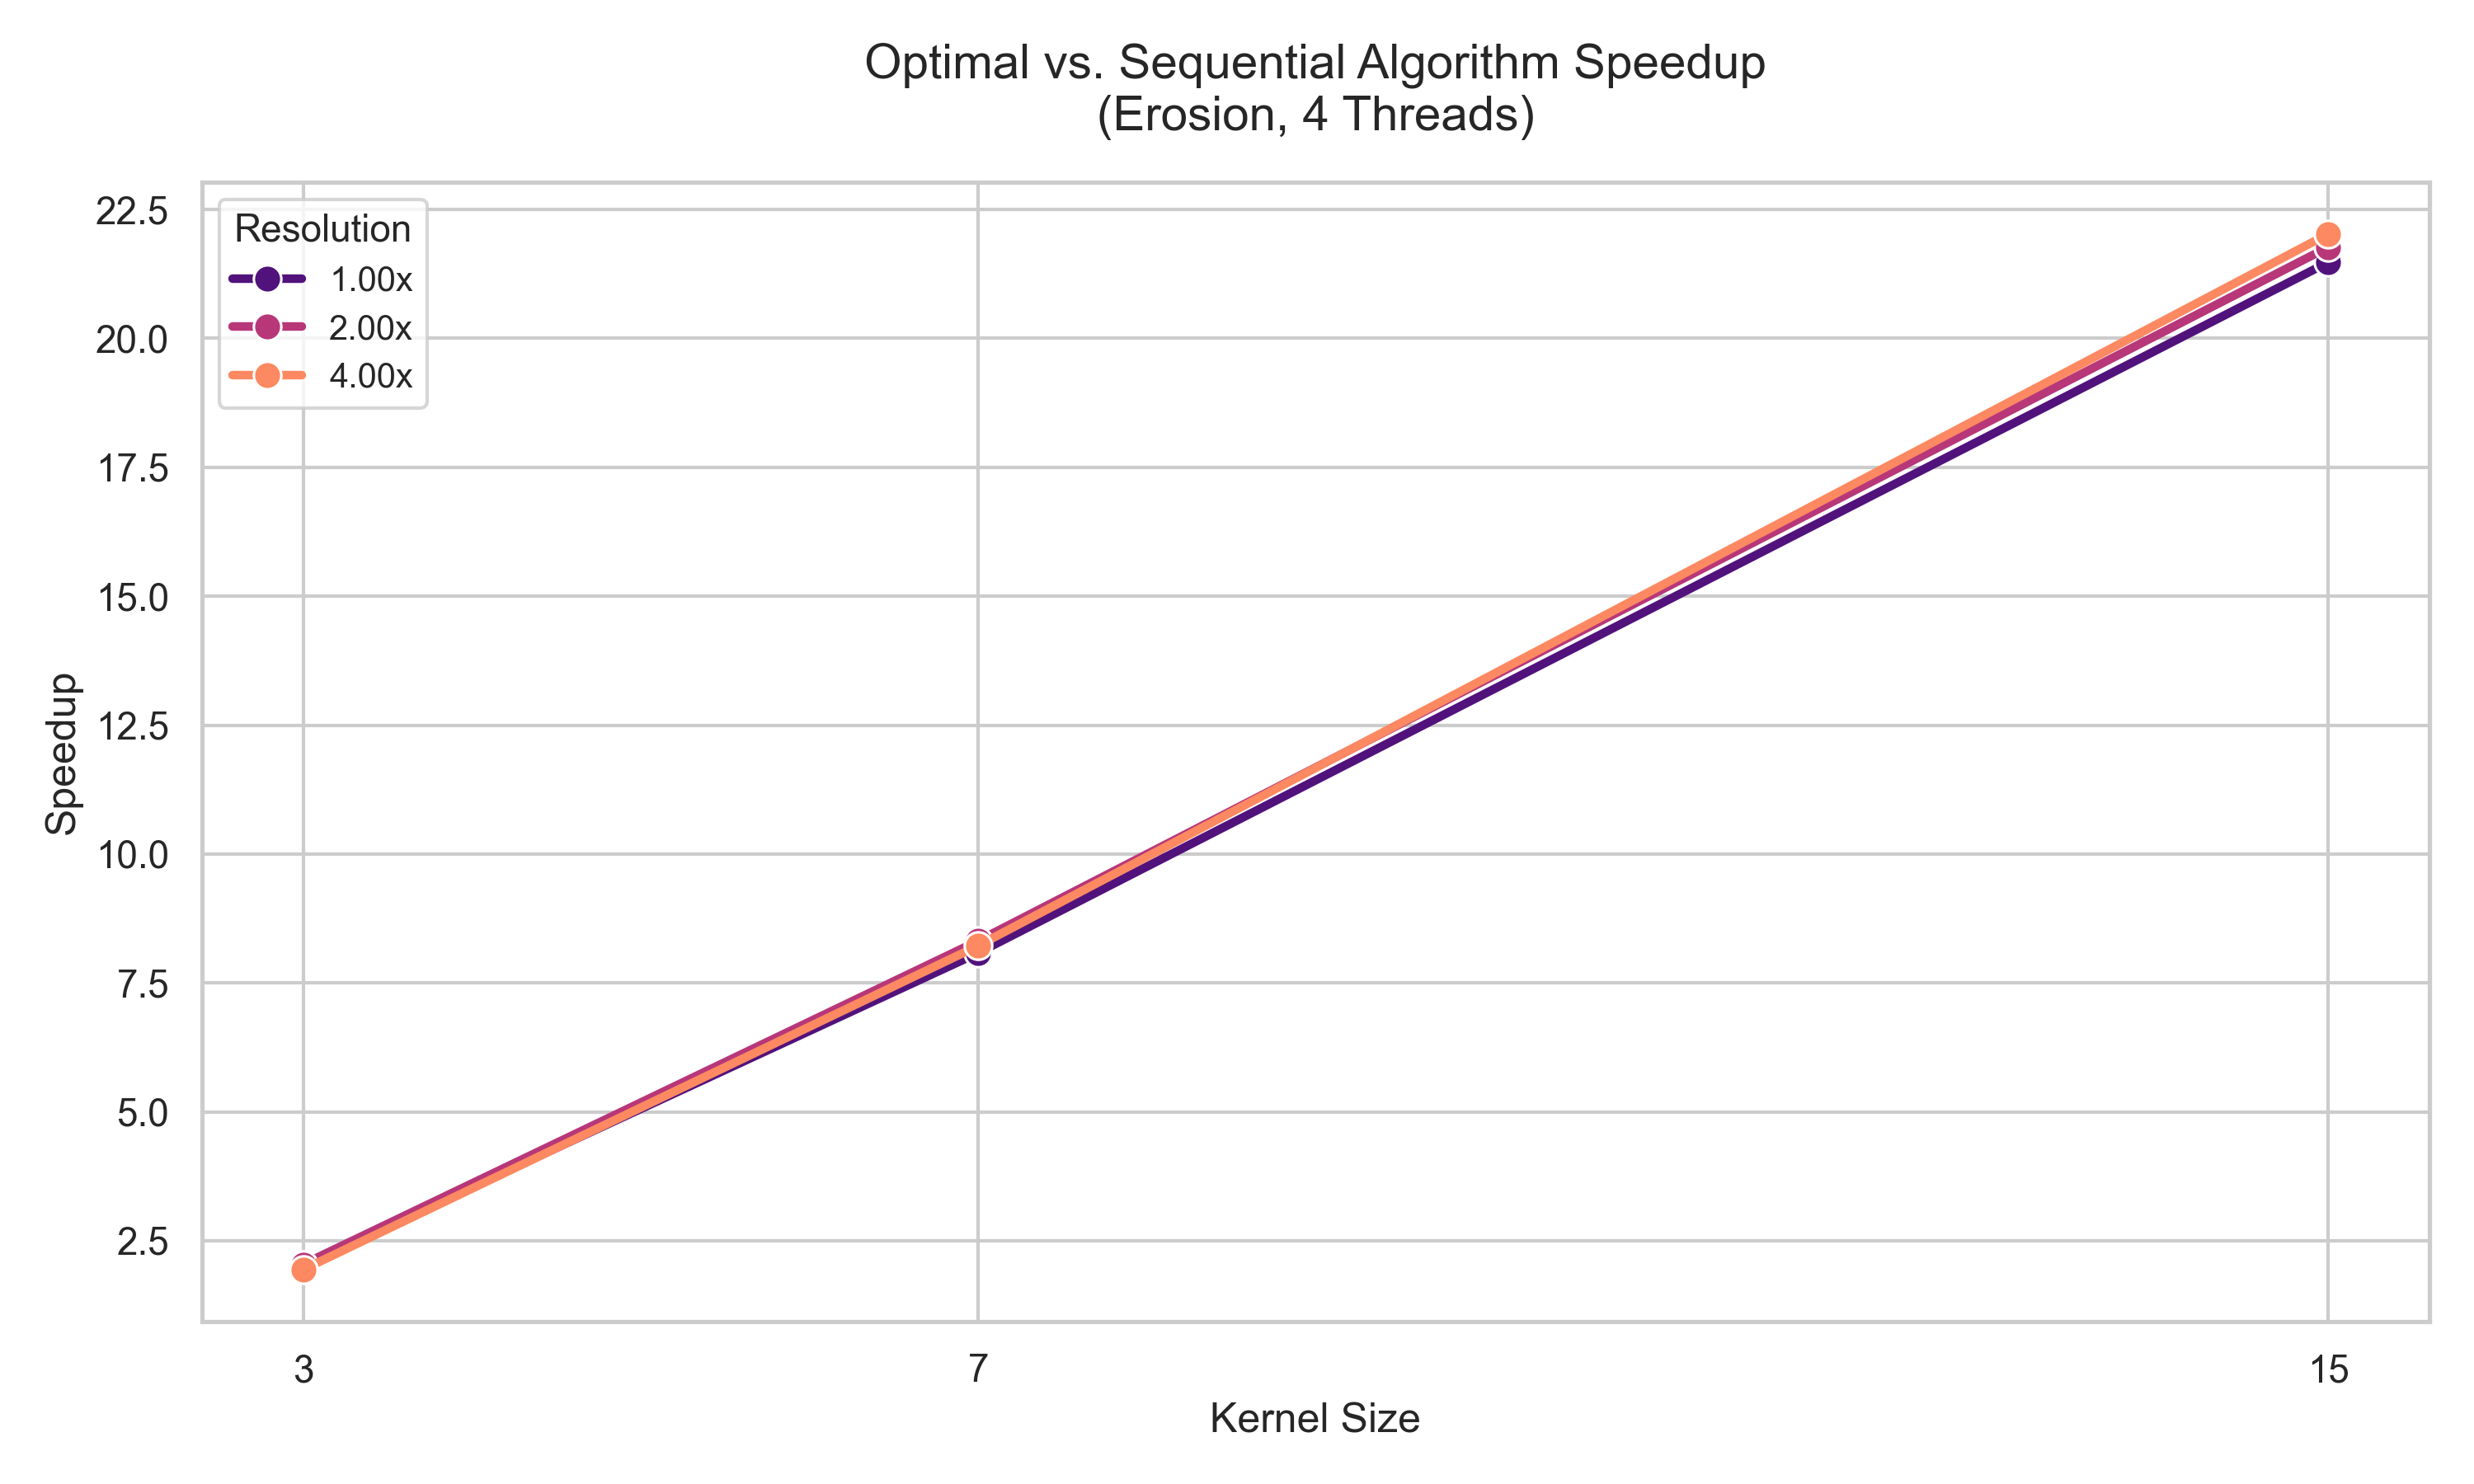
\includegraphics[width=0.85\linewidth]{img/optimal_speedup.png}
    \caption{Speedup of the optimal separable parallel implementation over the sequential 
    2D baseline, measured for Erosion across three image resolutions and kernel 
    sizes.}
    \label{fig:optimal_speedup}
\end{figure}


\subsection{Summary of Experimental Results}

The following tables consolidate the complete set of quantitative results 
obtained across all benchmark configurations. Each table corresponds to a 
distinct experimental axis investigated in this study. All speedup values 
are reported as mean $\pm$ 95\% confidence interval computed via Student's 
$t$-distribution over $N=5$ independent runs.


% ------------------------------------------------------------------
% TABLE 1: Separable Kernels (compatta)
% ------------------------------------------------------------------
\begin{table}[H]
\centering
\caption{Speedup of 1D Separable vs. 2D Parallel Baseline (4 threads).}
\label{tab:separable}
\renewcommand{\arraystretch}{1.15}
\begin{tabular}{cccc}
\hline
\textbf{Scale} & \textbf{K} & \textbf{Erosion} & \textbf{Dilation} \\
\hline
\multirow{3}{*}{2.0x} & 3  & $1.30 \pm 0.07$ & $1.71 \pm 0.13$ \\
                       & 7  & $3.11 \pm 0.20$ & $6.78 \pm 0.34$ \\
                       & 15 & $6.80 \pm 0.53$ & $13.43 \pm 0.29$ \\
\hline
\multirow{3}{*}{4.0x} & 3  & $1.23 \pm 0.06$ & $1.61 \pm 0.09$ \\
                       & 7  & $2.86 \pm 0.25$ & $5.86 \pm 0.44$ \\
                       & 15 & $6.57 \pm 0.14$ & $11.87 \pm 0.33$ \\
\hline
\end{tabular}
\end{table}

% ------------------------------------------------------------------
% TABLE 2: Optimal vs Sequential
% ------------------------------------------------------------------
\begin{table}[H]
\centering
\caption{Speedup of the optimal separable parallel implementation vs.\ the sequential 2D 
baseline, measured for Erosion.}
\label{tab:optimal}
\renewcommand{\arraystretch}{1.15}
\begin{tabular}{ccc}
\hline
\textbf{Scale} & \textbf{K} & \textbf{Speedup} \\
\hline
\multirow{3}{*}{1.0x} & 3  & $2.03 \pm 0.03$ \\
                       & 7  & $8.08 \pm 0.03$ \\
                       & 15 & $21.48 \pm 0.52$ \\
\hline
\multirow{3}{*}{2.0x} & 3  & $2.04 \pm 0.01$ \\
                       & 7  & $8.32 \pm 0.24$ \\
                       & 15 & $21.77 \pm 0.28$ \\
\hline
\multirow{3}{*}{4.0x} & 3  & $1.94 \pm 0.06$ \\
                       & 7  & $8.22 \pm 0.03$ \\
                       & 15 & $22.03 \pm 0.13$ \\
\hline
\end{tabular}
\end{table}

% ------------------------------------------------------------------
% TABLE 3: Pipeline Multi-Thread
% ------------------------------------------------------------------
\begin{table}[htbp]
\centering
\caption{Speedup of the Producer-Consumer pipeline vs.\ the standard 
parallel baseline for Opening and Closing ($K=7$).}
\label{tab:pipeline}
\renewcommand{\arraystretch}{1.15}
\begin{tabular}{cccc}
\hline
\textbf{Scale} & \textbf{Threads} & \textbf{Opening} & \textbf{Closing} \\
\hline
\multirow{3}{*}{1.0x} & 2 & $1.41 \pm 0.01$ & $1.39 \pm 0.02$ \\
                       & 4 & $1.26 \pm 0.10$ & $1.25 \pm 0.10$ \\
                       & 8 & $1.16 \pm 0.03$ & $1.19 \pm 0.03$ \\
\hline
\multirow{3}{*}{2.0x} & 2 & $1.52 \pm 0.00$ & $1.50 \pm 0.00$ \\
                       & 4 & $1.43 \pm 0.02$ & $1.43 \pm 0.02$ \\
                       & 8 & $1.33 \pm 0.02$ & $1.35 \pm 0.01$ \\
\hline
\end{tabular}
\end{table}
% ------------------------------------------------------------------
% TABLE 4: SIMD Impact
% ------------------------------------------------------------------
\begin{table}[H]
\centering
\caption{Impact of \texttt{\#pragma omp simd} on Erosion performance 
(scale 2.0x). Speedup $<1$ indicates a regression.}
\label{tab:simd}
\renewcommand{\arraystretch}{1.15}
\begin{tabular}{ccc}
\hline
\textbf{K} & \textbf{Threads} & \textbf{Speedup} \\
\hline
7  & 4 & $0.99 \pm 0.06$ \\
15 & 4 & $0.94 \pm 0.06$ \\
7  & 8 & $1.01 \pm 0.08$ \\
15 & 8 & $1.00 \pm 0.08$ \\
\hline
\end{tabular}
\end{table}

% ------------------------------------------------------------------
% TABLE 5: Scheduling Impact
% ------------------------------------------------------------------
\begin{table}[H]
\centering
\caption{Dynamic vs.\ static scheduling speedup on Erosion 
(scale 2.0x, $K=15$).}
\label{tab:scheduling}
\renewcommand{\arraystretch}{1.15}
\begin{tabular}{cc}
\hline
\textbf{Threads} & \textbf{Speedup} \\
\hline
4 & $1.06 \pm 0.09$ \\
8 & $1.07 \pm 0.08$ \\
\hline
\end{tabular}
\end{table}

% ------------------------------------------------------------------
% TABLE 6: Memory Access Pattern
% ------------------------------------------------------------------
\begin{table}[H]
\centering
\caption{Row-Major vs.\ Column-Major access pattern speedup 
($K=3$, parallel baseline).}
\label{tab:memory}
\renewcommand{\arraystretch}{1.15}
\begin{tabular}{ccc}
\hline
\textbf{Config} & \textbf{Operation} & \textbf{Speedup} \\
\hline
1T, 1.0x & Erosion  & $1.03 \pm 0.03$ \\
4T, 1.0x & Erosion  & $0.98 \pm 0.03$ \\
1T, 4.0x & Opening  & $0.95 \pm 0.02$ \\
4T, 4.0x & Dilation & $0.94 \pm 0.02$ \\
\hline
\end{tabular}
\end{table}

\section{Conclusions}
\label{sec:conclusions}
The experimental results align with theoretical predictions. 
The strong scaling analysis reflects the limits 
described by Amdahl's Law: the parallel speedup saturates around 
\textbf{3.5x--4.0x} at 4 physical cores, that is done by the hardware ceiling of 
the test machine and the residual sequential fraction 
of the execution.

This study demonstrates that achieving high performance on morphological image 
processing requires a multi-tiered optimization strategy. The compound effect 
of algorithmic reduction (1D separable kernels) and thread-level parallelism 
(\texttt{collapse(2)} and dynamic scheduling) yields a peak speedup of 
\textbf{22x} over the sequential baseline at $K=15$ with 4 threads, confirming 
that algorithmic complexity reduction is the dominant lever for performance. 
Additionally, the Producer-Consumer pipeline provides gains of up to 
\textbf{1.52x} for compound operations at low thread counts, while explicit 
SIMD annotations and column-major traversal prove ineffective in this context. 
As a potential development of the framework, extending it to 
support heterogeneous computing on GPUs via CUDA would offer greater scalability.

{\small
\bibliographystyle{ieee}
\bibliography{egbib}
}

\end{document}
